% **************************************************
% Document Class Definition
% **************************************************
\documentclass[%
    paper=A4,               % paper size --> A4 is default in Germany
    twoside=true,           % onesite or twoside printing
    openright,              % doublepage cleaning ends up right side
    parskip=full,           % spacing value / method for paragraphs
    chapterprefix=true,     % prefix for chapter marks
    11pt,                   % font size
    headings=normal,        % size of headings
    bibliography=totoc,     % include bib in toc
    listof=totoc,           % include listof entries in toc
    titlepage=on,           % own page for each title page
    captions=tableabove,    % display table captions above the float env
    draft=false,            % value for draft version
]{scrreprt}%

% !TEX root = main.tex


% **************************************************
% Files' Character Encoding
% **************************************************
\PassOptionsToPackage{utf8}{inputenc}
\usepackage{inputenc}
\usepackage[english,ngerman]{babel}

% **************************************************
% Information and Commands for Reuse
% **************************************************
\newcommand{\thesisTitle}{Probabilistische online Wissensgraphkonstruktion aus natürlicher Sprache}
\newcommand{\thesisName}{Clemens Damke}
\newcommand{\thesisMatNr}{7011488}
\newcommand{\thesisSubject}{Bachelorarbeit}
\newcommand{\thesisDate}{\today}
\newcommand{\thesisVersion}{Entwurf 1}

\newcommand{\thesisFirstReviewer}{Prof.~Dr.~Eyke Hüllermeier}
\newcommand{\thesisFirstReviewerUniversity}{\protect{Universität Paderborn}}
\newcommand{\thesisFirstReviewerDepartment}{Institut für Informatik}

\newcommand{\thesisSecondReviewer}{Prof.~Dr.~Axel-Cyrille Ngonga Ngomo}
\newcommand{\thesisSecondReviewerUniversity}{\protect{Universität Paderborn}}
\newcommand{\thesisSecondReviewerDepartment}{Institut für Informatik}

\newcommand{\thesisFirstSupervisor}{Dr.~Theodor Lettmann}
\newcommand{\thesisSecondSupervisor}{Prof.~Dr.~Eyke Hüllermeier}

\newcommand{\thesisUniversity}{Universität Paderborn}
\newcommand{\thesisUniversityDepartment}{}
\newcommand{\thesisUniversityInstitute}{Institut für Informatik}
\newcommand{\thesisUniversityGroup}{Intelligente Systeme}
\newcommand{\thesisUniversityCity}{Paderborn}
\newcommand{\thesisUniversityStreetAddress}{Pohlweg 51}
\newcommand{\thesisUniversityPostalCode}{33098}


% **************************************************
% Debug LaTeX Information
% **************************************************
%\listfiles


% **************************************************
% Load and Configure Packages
% **************************************************

% Colors:
\usepackage[usenames, dvipsnames, svgnames, table]{xcolor}

\definecolor{blau}{HTML}{355FB3}
\definecolor{rot}{HTML}{B33535}
\definecolor{gruen}{HTML}{3BB335}
\definecolor{dunkelblau}{HTML}{1E3666}
\definecolor{hellblau}{HTML}{8ea7d7}

\PassOptionsToPackage{% setup clean thesis style
    figuresep=space,
    sansserif=false,
    hangfigurecaption=false,
    hangsection=true,
    hangsubsection=true,
    colorize=full,
    colortheme=custom,
	colormain=dunkelblau,
	coloraccessory=blau,
    bibsys=bibtex,
    bibfile=bib-refs,
    bibstyle=alphabetic,
    wrapfooter=false,
}{cleanthesis}
\usepackage{cleanthesis}

\usepackage{mathtools}
\newcommand\numberthis{\addtocounter{equation}{1}\tag{\theequation}}

\usepackage{stmaryrd}

\usepackage{tikz}
\usetikzlibrary{calc}
\newcommand{\tikzmark}[1]{\tikz[overlay,remember picture] \node (#1) {};} % chktex 1

\usepackage[bguq]{frege}

\usepackage{pgfplots}
\usepackage{pgfplotstable}
\pgfplotsset{compat=1.14}
\usepgfplotslibrary{dateplot, statistics}
\pgfplotsset{
    cycle list={blau\\rot\\gruen\\},
}

\hypersetup{% setup the hyperref-package options
    pdftitle={\thesisTitle},    %   - title (PDF meta)
    pdfsubject={\thesisSubject},%   - subject (PDF meta)
    pdfauthor={\thesisName},    %   - author (PDF meta)
    plainpages=false,           %   -
    colorlinks=false,           %   - colorize links?
    pdfborder={0 0 0},          %   -
    breaklinks=true,            %   - allow line break inside links
    bookmarksnumbered=true,     %
    bookmarksopen=true          %
}


% **************************************************
% Document CONTENT
% **************************************************
\begin{document}

% --------------------------
% rename document parts
% --------------------------
\renewcaptionname{ngerman}{\figurename}{Abb.}
\renewcaptionname{ngerman}{\tablename}{Tab.}

% --------------------------
% Front matter
% --------------------------
\pagenumbering{roman}			% roman page numbing (invisible for empty page style)
\pagestyle{empty}				% no header or footers
% !TEX root = ../main.tex
%
% ------------------------------------  --> cover title page
\begin{titlepage}
	\pdfbookmark[0]{Cover}{Cover}
	\flushright\
	\hfill
	\vfill
	{\LARGE\thesisTitle\ \par}
	\rule[5pt]{\textwidth}{.4pt} \par
	{\Large\thesisName}
	\vfill
	\textit{\large\thesisDate} \\
	Version: \thesisVersion\
\end{titlepage}


% ------------------------------------  --> main title page
\begin{titlepage}
	\pdfbookmark[0]{Titlepage}{Titlepage}
	\tgherosfont\

	\begin{figure}
	\begin{minipage}[t]{8.5cm}
	
\includegraphics[height=1.8cm]{gfx/upb_1E}\\
	\textsf{\small{\hspace*{1.3cm}Department of Electrical Engineering,\\
	\hspace*{1.3cm}Computer Science and Mathematics\\
%		\hspace*{1.3cm}Institute of Computer Science\\
		\hspace*{1.3cm}Warburger Straße 100 \\
		\hspace*{1.3cm}33098 Paderborn
		}}
	\end{minipage}
	\hfill
	\begin{minipage}[t]{4.7cm}
	
\includegraphics[height=1.8cm]{gfx/is-logo-klein}\\
	\textsf{%Institute of Computer Science\\
	\hspace*{0.1cm}\small{Intelligent Systems Group (ISG)}
	}
	\end{minipage}
	\end{figure}

	\centering
	%\textsf{\thesisUniversityDepartment} \\
	%\textsf{\thesisUniversityInstitute} \\
	%\textsf{\thesisUniversityGroup} \\

	\vfill
	{\large \thesisSubject} \\[5mm]
	{\LARGE \color{ctcolortitle}\textbf{\thesisTitle} \\[10mm]}
	{\Large \thesisName} \\

	\vfill
	\begin{minipage}[t]{.27\textwidth}
		\raggedleft\
		\textit{1. Korrektor}
	\end{minipage}
	\hspace*{15pt}
	\begin{minipage}[t]{.65\textwidth}
		{\Large \thesisFirstReviewer} \\
	  	{\small \thesisFirstReviewerDepartment} \\[-1mm]
		{\small \thesisFirstReviewerUniversity}
	\end{minipage} \\[5mm]
	\begin{minipage}[t]{.27\textwidth}
		\raggedleft\
		\textit{2. Korrektor}
	\end{minipage}
	\hspace*{15pt}
	\begin{minipage}[t]{.65\textwidth}
		{\Large \thesisSecondReviewer} \\
	  	{\small \thesisSecondReviewerDepartment} \\[-1mm]
		{\small \thesisSecondReviewerUniversity}
	\end{minipage} \\[10mm]
	\begin{minipage}[t]{.27\textwidth}
		\raggedleft\
		\textit{Betreuer}
	\end{minipage}
	\hspace*{15pt}
	\begin{minipage}[t]{.65\textwidth}
		\thesisFirstSupervisor\ und \thesisSecondSupervisor\
	\end{minipage} \\[10mm]

	\thesisDate\\ % chktex 21

\end{titlepage}


% ------------------------------------  --> lower title back for single page layout
\hfill
\vfill
{
	\small
	\textbf{\thesisName} \\
	\textit{\thesisTitle} \\
	\thesisSubject, \thesisDate\\ % chktex 21
	Korrektoren: \thesisFirstReviewer\ und \thesisSecondReviewer\\ % chktex 21
	Betreuer: \thesisFirstSupervisor\ und \thesisSecondSupervisor\\[1.5em] % chktex 21
	\textbf{\thesisUniversity} \\
	\textit{\thesisUniversityGroup} \\
	\thesisUniversityInstitute\\ % chktex 21
	\thesisUniversityDepartment\\ % chktex 21
	\thesisUniversityStreetAddress\\ % chktex 21
	\thesisUniversityPostalCode\ \thesisUniversityCity\
}
		% INCLUDE: all titlepages
\cleardoublepage\

\pagestyle{plain}				% display just page numbers
% !TEX root = ../my-thesis.tex
%
\pdfbookmark[0]{Abstract}{Abstract}
\chapter*{Abstract}
\label{sec:abstract}
\vspace*{-10mm}

\blindtext

\vspace*{20mm}

{\usekomafont{chapter}Abstract (different language)}\label{sec:abstract-diff} \\

\blindtext
		% INCLUDE: the abstracts (english and german)
\cleardoublepage\
%
\setcounter{tocdepth}{2}		% define depth of toc
\tableofcontents				% display table of contents
\cleardoublepage\

% --------------------------
% Body matter
% --------------------------
\pagenumbering{arabic}			% arabic page numbering
\setcounter{page}{1}			% set page counter
\pagestyle{maincontentstyle} 	% fancy header and footer

% !TEX root = ../main.tex
% chktex-file 46
\chapter{Einleitung}%
\label{sec:intro}

\cleanchapterquote{
The actual world cannot be distinguished from a world of imagination by any description.
Hence the need of pronoun and indices, and the more complicated the subject the greater the need of them.
}{Charles Sanders Peirce}{Mathematiker und Philosoph}

\section{Motivation}%
\label{sec:intro:motivation}

In den letzten Jahren hat die Repräsentation von Wissensbasen durch Graphen, sog. Wissensgraphen, immer mehr an Bedeutung gewonnen.
Google, Bing und IBM Watson benutzen solche Wissensgraphen z.~B. zum Beantworten von komplexen Suchanfragen.

Die Grundidee dabei ist es, Entitäten durch Knoten und Relationen durch Kanten abzubilden.
Entitäten können konkrete Dinge, wie z.~B. Personen, aber auch abstrakte Konzepte, wie z.~B. historische Epochen, sein.
Relationen beschreiben beliebige Beziehungen zwischen den Entitäten, z.~B. $person(\text{Da~Vinci}) \xrightarrow{\text{lived~in}} epoch(\text{Renaissance})$.
Die Entität, von der eine solche Relation ausgeht, wird als Subjekt und die Zielentität als Objekt der Relation bezeichnet.

Die Typen von Entitäten bzw.\ Relationen (z.~B. $person$ bzw. $lived~in$) und deren Bedeutung sind dabei i.~d.~R. formal in einer sog.\ Ontologie spezifiziert.
Die Ontologie beschränkt also die Menge gültiger Wissensgraphen, was eine effiziente maschinelle Verarbeitung der im Graph enthaltenen Informationen ermöglicht.

Da Wissensgraphen in zahlreichen Domänen einsetzbar sind, wird deren automatisierte Konstruktion bereits seit Jahren erforscht.
Manuelles Konstruieren und vor allem anschließendes Warten und Aktualisieren von Wissensgraphen, ist aufgrund der abzubildenden Datenmengen nicht praktikabel.
Bei einer maschinellen automatisierten Konstruktion sind insbesondere zwei Anforderungen problematisch:
\begin{enumerate}
	\item Das Verarbeiten von unstrukturierten Eingaben, wie z.~B. natürlichsprachlichen Texten.
	\item Effizientes Eingliedern neuer Informationen in einen bestehenden Wissensgraphen.
		Dieses Eingliedern von Informationen umfasst im Speziellen:
		\begin{itemize}
			\item \textbf{Entity Resolution:}
				Hinzukommende Entitäten, die bereits im Graphen enthalten sind, müssen als Duplikate erkannt werden.
				Dies ist i.~d.~R. nicht trivial, da die selbe Entität durch viele verschiedene, oftmals vom Kontext abhängige, Token repräsentiert werden kann;
				z.~B. \textit{Bob} vs. \textit{Robert} oder \textit{Der Papst} vs. \textit{Franziskus}.
			\item \textbf{Link Prediction:}
				Hinzukommende Entitäten müssen mit bereits bestehenden Entitäten in Relation gesetzt werden.
				Hinzukommende Relationen können zudem benutzt werden um andere Relationen zu inferieren;
				z.~B. \[female(A) \land B \xrightarrow{\text{son~of}} A \implies A \xrightarrow{\text{mother~of}} B\]
		\end{itemize}
\end{enumerate}

Die Kombination dieser beiden Anforderungen ist interessant, da das meiste verfügbare Wissen in natürlichsprachlicher Textform vorliegt und zudem permanent neues Wissen entsteht.
Ein automatisiertes Wissensgraphkonstruktionsverfahren, welches beide Anforderungen berücksichtigt, ist daher in diversen Domänen von Nutzen.
Ein Beispiel hierfür ist die Auswertung von Kommunikationsdaten aus E-Mails oder Chat-Nachrichten mit dem Ziel die sozialen Beziehungen und Intentionen der Kommunikationpartner zu ermitteln.

\section{Ziele der Arbeit}%
\label{sec:intro:goals}

Das übergeordnete Ziel dieser Arbeit ist es, ein Verfahren zu finden, welches das soeben beschriebene Problem der automatisierten Wissensgraphkonstruktion für E-Mail-Daten löst.
Konkret sei ein Stream von E-Mails gegeben, denen jeweils ein Inhalt, ein Absender, eine Menge von Empfängern und ggf.\ weitere Metadaten, wie z.~B. Absendezeit, Absendeort oder IP-Adresse, zugeordnet ist.
Die Nachrichteninhalte werden der Einfachheit halber als ausschließlich englischsprachig angenommen.
Außerdem wird eine, für E-Mails und andere Kurznachrichten typische, eingeschränkte Sprachkomplexität angenommen.
Die Nachrichten sollen nacheinander in das zu konstruierende System eingefügt werden, welches sukzessive einen Wissensgraphen daraus erzeugt.

Für diese Erzeugung muss eine Reihe von Teilproblemen gelöst werden:
\begin{enumerate}
	\item \textbf{Onotologie:}
		Spezifikation einer Wissensgraphontologie, die mächtig genug ist, um die Diversität natürlichsprachlich beschriebener Informationen abzubilden.
	\item \textbf{Repräsentation:}
		Spezifikation der maschinellen Repräsentation des Wissensgraphen.
	\item \textbf{Sprachverarbeitung:}
		Finden eines Verfahrens, welches die natürlichsprachlichen Inhalte der Nachrichten in eine für die Wissensgraphkonstruktion geeignete Form bringt.
	\item \textbf{Grapherweiterung:}
		Finden eines Verfahrens, um eine eintreffende Nachricht in den bestehenden Wissensgraphen einzufügen.
\end{enumerate}

Das aus den Teillösungen zusammengesetzte Verfahren muss, neben der offensichtlichen Anforderung einen Wissensgraphen zu konstruieren, zudem folgende technische Anforderungen erfüllen:
\begin{enumerate}
	\item \textbf{Erweiterbarkeit:}
		Es sollen Schnittstellen eingeplant sein, um neben der Sprachverarbeitung auch andere Verarbeitungsverfahren, z.~B. für Bilder, hinzufügen zu können.
		Die Graphontologie, Graphrepräsentation und das Grapherweiterungsverfahren dürfen also nicht zu sehr auf die Struktur natürlicher Sprache zugeschnitten sein.
	\item \textbf{Parallelisierbarkeit:}
		Das Verfahren soll in der Lage sein die Rechenleistung mehrerer Prozessorkerne zu nutzen.
		Diese Anforderung betrifft insbesondere das Grapherweiterungsverfahren.
\end{enumerate}

\section{Aufbau der Arbeit}%
\label{sec:intro:structure}

\paragraph{Kapitel~\ref{sec:related}}

\paragraph{Kapitel~\ref{sec:theory}}

\paragraph{Kapitel~\ref{sec:text2kg}}

\paragraph{Kapitel~\ref{sec:evaluation}}

\paragraph{Kapitel~\ref{sec:conclusion}}

% !TEX root = ../main.tex
% chktex-file 46
\chapter{Verwandte Arbeiten}%
\label{sec:related}

Die in~\ref{sec:intro:goals} beschriebenen Ziele werden bereits seit langem erforscht.
Der Begriff \textit{Wissensgraph} wurde 2012 durch Google popularisiert, die Ideen dahinter lassen sich allerdings bis ins Ende des 19. Jahrhunderts zurückverfolgen.
Dieses Kapitel zeigt auf, wie sich die Themen dieser Arbeit in die bisherige Forschung einfügen.
\ref{sec:related:kr} ordnet hierfür das Konzept des Wissensgraphen in die Entwicklungsgeschichte der Wissensrepräsentation ein. % chktex 2
In~\ref{sec:related:nlp} wird ein Überblick über die momentan verbreiteten \textit{Natural Language Processing} (NLP) Werkzeuge gegeben.
Das Wissensgraphkonzept und NLP wird schließlich in~\ref{sec:related:kgc} kombiniert und es werden die aktuell verwendeten Verfahren zur Wissensgraphkonstruktion beschrieben.

\section{Ansätze zur Wissensrepräsentation}%
\label{sec:related:kr}

\subsection{Logische Grundlagen}%
\label{sec:related:kr:logic}

Die Entwicklung der Wissensrepräsentation hängt eng mit der Entwicklung der Logik zusammen.
Während in der formalen Logik und Mathematik die Prädikatenlogik das allgemein verwendete Kalkül ist und alternative Formalismen kaum verbreitet sind, finden im Bereich der Wissensrepräsentation bis heute diverse andere Kalküle Verwendung.
Diese werden im Folgenden kurz vorgestellt.

\paragraph{Begriffsschrift (1879)}
Gottlob Freges Buch über die \textit{Begriffsschrift}~\cite{Frege1879} gilt als eines der bedeutsamsten Werke der Logik.
Sie ist der erste Formalismus mit der Mächtigkeit der modernen Prädikatenlogik zweiter Ordnung mit Identität.
Frege benutzt hierfür eine zweidimensionale Notation, die sich stark von der heute gebräuchlichen, linearen, an die Algebra angelehnte Notation unterscheidet.
\begin{equation*}
	\vcenter{\hbox{\Fconditional[\Fanqn{a}]{\Fcontent \mathfrak{R(a)}}{\Fncontent \mathfrak{P(a)}}}}
	\quad\Leftrightarrow\quad
	\exists\ a: P(a) \lor R(a)
\end{equation*}
Im Gegensatz zur Prädikatenlogik gibt es keine eigene Syntax für \textit{UND} und \textit{ODER};
diese Operatoren müssen durch die Kombination von Negation und Implikation abgebildet werden.
Zudem gibt es ausschließlich den Allquantor;
eine existenzquantisierte Aussage muss durch Negation der negierten allquantisierten Aussage ausgedrückt werden.

\paragraph{Prädikatenlogik: Peirce Notation (1885)}
Unabhängig von Frege entwickelte der amerikanische Mathematiker Charles Sanders Peirce ebenfalls ein prädikatenlogisches Kalkül~\cite{Peirce1885}.
Peirces Notation hatte starke Ähnlichkeiten mit der heute benutzten linearen Schreibweise.
Statt den modernen Symbolen hat Peirce allerdings die algebraischen Operatoren benutzt, um die Analogien zwischen Logik und Algebra auszudrücken.
\begin{equation*}
	\Sigma_a\ P_a + R_a
	\quad\Leftrightarrow\quad
	\exists\ a: P(a) \lor R(a)
\end{equation*}

\paragraph{Existential Graphs (1897)}
Neben seiner zuvor entwickelten linearen prädikatenlogischen Notation, hat Peirce zudem viele Jahre an einem alternativen graphischen Kalkül gearbeitet, welches er \textit{Existential Graphs} (zu dt.~Existenzgraphen)~\cite{Sowa2011} nannte.
Ähnlich wie die Begriffsschrift werden Existenzgraphen zweidimensional dargestellt.
Von dieser Gemeinsamkeit abgesehen, funktionieren sie allerdings fundamental verschieden.
Ein logischer Ausdruck wird hier durch einen ungerichteten Graphen beschrieben.
Die konkrete räumliche Anordnung der Knoten und Kanten hat dabei keine semantische Relevanz.

Peirce hat Existenzgraphen als ein dreistufiges aufeinander aufbauendes System konzipiert.
Die erste Stufe, die sog.\ $\alpha$-Graphen, umfasst alle notwendigen syntaktischen Elemente, um ein Kalkül mit der Mächtigkeit der Aussagenlogik zu erhalten.
Die $\beta$-Graphen bilden die zweite Stufe und erweitern die Syntax der $\alpha$-Graphen, sodass die Mächtigkeit der Prädikatenlogik erster Ordnung erreicht wird.
Sowohl für $\alpha$-, als auch für $\beta$-Graphen, ist die Vollständigkeit und Korrektheit bewiesen.
Die dritte Stufe ($\gamma$-Graphen) wurde von Pierce nie vollendet;
sie deckt in etwa die Mächtigkeit der heutigen Prädikatenlogik höherer Ordnung sowie der Modallogik ab.
\begin{align*}
	\vcenter{\hbox{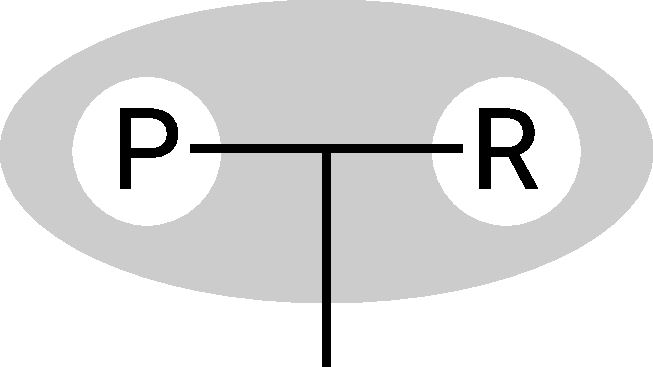
\includegraphics[height=3em]{gfx/related-work/existentialGraphExample1.pdf}}}
	\quad\Leftrightarrow\quad
	\exists\ a: P(a) \lor R(a)
\end{align*}
Wie schon die Begriffsschrift, sind Existenzgraphen syntaktisch minimal.
Direkt ausdrücken lässt sich lediglich \textit{UND}, der Existenzquantor und die Negation.
Ein weiterer Unterschied zur heutigen Prädikatenlogik ist die Beschreibung logischer Inferenzen.
Im Gegensatz zu den prädikatenlogischen Ersetzungsaxiomen, die auf der syntaktischen Struktur von logischen Ausdrücken operieren (z.~B. für Kommutativität), lassen sich die Ersetzungsaxiome für Existenzgraphen als Graphtransformationsregeln verstehen, die bestimmte Teilmengen der Knoten und Kanten eines Ausdrucks durch andere äquivalente Knoten- und Kantenmengen ersetzen.

\paragraph{Prädikatenlogik: Peano-Russell Notation (1910)}
Die zweidimensionalen Notationen wurde häufig kritisiert, da sie die lineare, algebraische Notation der symbolischen Logik von Boole und De Morgan verwarfen~\cite{Sluga1987}.
Freges Begriffsschrft und Peirces Existenzgraphen konnten sich daher nicht durchsetzen.
Peirces algebraische prädikatenlogische Notation hingegen, stieß auf größere Akzeptanz.
Giuseppe Peano hat auf deren Basis eine ähnliche Notation entwickelt, welche allerdings nicht die algebraischen Operatoren benutzt, damit sich logische Ausdrücke besser mit mathematischen Ausdrücken kombinieren lassen.
Bertrand Russell hat Peanos Notation anschließend in leicht abgewandelter Form in den \textit{Principia Mathematica}~\cite{Whitehead1910} benutzt.
Diese sog.~Peano-Russell-Notation ist im Wesentlichen identisch mit der modernen Schreibweise.

Trotz des Verschwindens der zweidimensionalen Notationen, finden sich noch heute Anlehnungen daran~\cite{WikiBegriffsschrift}.
So ist z.~B. die Negation $\lnot A$ auf Freges negierten Inhaltsstrich $\Fncontent A$ und der Ableitungsoperator $\vdash$ auf Freges Urteilsstrich mit angefügtem Inhaltsstrich $\Facontent$ zurückzuführen.

\subsection{Entwicklung maschineller Wissensrepräsentation}%
\label{sec:related:kr:history}

Die Idee Computer zur Lösung beliebiger Probleme zu benutzen ist nicht neu.
Da ein solches maschinelles Problemlösen die Verfügbarkeit von Hintergrundwissen über die Problemdomäne erfordert,
wurden Methoden zur Wissensrepräsentation immer im Zusammenhang mit Problemlösern erforscht.
So wie effiziente Datenstrukturen die Implementation effizienter Algorithmen ermöglichen, ermöglichen gute Wissensrepräsentationen die Implementation guter Problemlöser.
Was genau nun als ein guter Problemlöser verstanden wird, hat sich im Laufe der Jahre allerdings immer wieder verändert.

\paragraph{Universelle Problemlöser}
Einer der ersten maschinellen Problemlöser war der von Simon, Shaw und Newell 1955 entwickelte \textit{Logic Theorist} (LT).
LT war in der Lage logische Aussagen zu beweisen, indem er systematisch Ersetzungsaxiome auf eine gegebene Aussage angewandt hat, bis die gesuchte Lösung abgeleitet wurde.

Die Grundidee des LT haben Simon, Shaw und Newell 1959 im \textit{General Problem Solver} (GPS) erweitert.
Es wurden Heuristiken hinzugefügt, um den Suchraum geschickter zu durchlaufen.
GPS war ein universeller Problemlöser, konnte also jedes Problem lösen, das sich durch eine Menge von Horn-Klauseln ausdrücken lässt.
Zwar war es so theoretisch möglich Probleme aus diversen Domänen zu lösen, aufgrund der kombinatorischen Explosion war GPS alledings nicht zur Lösung komplexer praktischer Probleme geeignet.

\paragraph{Expertensysteme}
Aufgrund der Misserfolge universeller Problemlöser für praktische Probleme, hat die Forschung begonnen sich mehr auf die Entwicklung von Expertensystemen zu fokussieren.
Expertensysteme besitzen für gewöhnlich eine Wissensbasis in der domänenspezifisches Wissen in Form von Regeln und Fakten kodiert ist.
Eine sog.~Inferenzmaschine benutzt diese Regeln und Fakten um Probleme zu lösen.

\paragraph{Semantic Networks (1956)}
Die Idee, Graphen als Datenstruktur für Wissensbasen zu verwenden, taucht erstmal in den sog.~\textit{Semantic Networks} (zu dt.~semantische Netzwerke) auf.
Dieser Ansatz beschreibt Wissen als Menge von $(subject, predicate, object)$-Tripeln.
Es gibt darüber hinaus allerdings keine klaren Regeln, wie ein semantisches Netz strukturiert sein muss.
Semantische Netzwerke sind daher allenfalls als ein Oberbegriff für die große Vielfalt konkreter graphbasierter Wissensbasen zu verstehen.

\paragraph{Conceptual Graphs (1976)}
Wie genau mit Graphen komplexes Wissen beschrieben werden kann, das über eine reine Taxonomie hinaus geht, blieb bei semantischen Netzen unklar.
John F. Sowas \textit{Conceptual Graphs} (zu dt.~Konzeptgraphen) lösen dieses Problem.
Statt Wissen lediglich als eine einfache Menge von Beziehungen abzubilden, wird es als prädikatenlogischer Ausdruck verstanden.
Hierfür baut Sowa auf Peirces Existenzgraphen auf, die bis dahin weitestgehend unbeachtet waren.
\begin{align*}
	\vcenter{\hbox{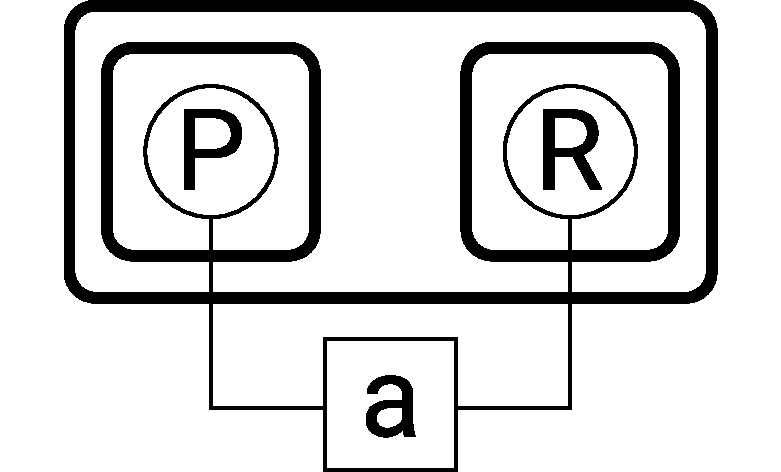
\includegraphics[height=4em]{gfx/related-work/conceptGraphExample1.pdf}}}
	\quad\Leftrightarrow\quad
	\exists\ a: P(a) \lor R(a)
\end{align*}
Dieser Ansatz erlaubt es komplexe Wissensbasen zu konstruieren, in denen nicht nur gespeichert werden kann, ob ein Konzept existiert, sondern auch, ob es nicht oder nur möglicherweise existiert.
Da Konzeptgraphen, so wie schon die Existenzgraphen, ein vollständiges und korrektes Logikkalkül sind, lassen sich zudem Inferenzregeln für sie definieren.
Der Vorteil hierfür einen Graphen statt eines prädikatenlogischen Ausdrucks zu verwenden ist, dass eine Graphstruktur einen deutlich effizienteren Zugriff auf gespeichertes Wissen ermöglicht.

\paragraph{Knowledge Graphs (1987)}
Der Begriff \textit{Knowledge Graph} (zu dt.~Wissensgraph) bezeichnete ursprünglich eine Klasse semantischer Netze, deren Relationsmenge formal spezifiziert ist.
Dies schränkt die Menge erlaubter Graphen ein und ermöglicht die Definition von Inferenzregeln, um Schlussfolgerungen aus einem gegebenen Graphen zu ziehen.
Im Laufe der Jahre ist die Grenze zwischen semantischen Netzen und Wissensgraphen allerdings immer weiter verschwommen, sodass die Bezeichnungen heute oft synonym verwendet werden.
Wissensgraphen und Konzeptgraphen müssen weiterhin unterschieden werden, da erstere oftmals Negation und Modalität nicht unterstützen.

\subsection{Aktuelle Wissensrepräsentationsprojekte}%
\label{sec:related:kr:today}

\subsubsection{Manuelle Ansätze}

\paragraph{Semantic Web}
Das sog.~\textit{Semantic Web} bezeichnet eine Menge von W3C-Standards, die das bestehende Web um eine formale Wissensbeschreibungssyntax erweitern.
Zentral ist dabei das \textit{Resource Description Framework} (RDF), mit dem sich beliebige Konzepte, auch Resourcen genannt, beschreiben und verknüpfen lassen.
Ziel ist es über die unstrukturierte Netzstruktur des bestehenden Webs, eine strukturierte, leicht maschniell verarbeitbare, Netzstruktur zu legen.
Durch die Anfragesprache \textit{SPARQL} ist es möglich Wissen aus diesem Netz auszulesen.
Das Web würde somit zu einem großen denzentralen Wissensgraphen.
Tim Berners-Lee beschreibt diese Idee als das ``Web 3.0''.
Obwohl die Technologien hierfür bereits seit Jahren existieren, sind bislang nur wenige Webseiten mit RDF-Tags annotiert.
Häufige Kritik ist, dass das Semantic Web zu viel theoretisches Hintergrundwissen über Wissensrepräsentationsverfahren erfordert, um für die meisten Webseitenbetreiber zugänglich zu sein.

\paragraph{WordNet}
Das \textit{WordNet} der Universität Princeton ist ein frei verfügbares lexikalisch-semantisches Netz für die englische Sprache, d.~h.\ ein semantisches Netz, welches die Bedeutung von Worten in Relation zueinander setzt.
Relationen werden dabei z.~B. für Synonyme, Hypernyme (Oberbegriffe) und Meronyme (Bestandteile) eingefügt.
Der Datenbestand des WordNets wird manuell gepflegt und resultiert aus der Kombination der Einträge verschiedener Wörterbücher.

\subsubsection{Automatisierte Ansätze}
Neben den manuellen Grapherzeugungsansätzen des Semantic Webs und des WordNets, gibt es diverse voll- und semiautomatische Ansätze.
Diese bauen die Graphstruktur selbstständig aus gegebenen Datenquellen auf.

\paragraph{NELL}
Das \textit{Never-Ending Language Learning} (NELL) System traviersiert selbstständig das Internet und fügt die gefundenen textuellen Informationen in einen Wissensgraphen ein.
Hierfür wird eine Kombination verschiedener Modelle verwendet, die regelmäßig angepasst wird.
Menschen können optional Feedback für die extrahierten Fakten geben, um die Inferenzqualität weiter zu verbessern.

\paragraph{Google Knowledge Graph}
Basierend auf den Ideen der in~\ref{sec:related:kr:history} vorgestellten Wissensgraphen, stellte Google 2012 eine eigene, ebenfalls \textit{Knowledge Graph} genannte, Wissensgraphtechnologie vor~\cite{Singhal2012}.
Sie wird benutzt, um Suchanfragen semantisch, statt per String-Matching, zu beantworten.
So können z.~B. zum Suchbegriff verwandte Ergebnisse angezeigt werden, selbst wenn es keine textuelle Ähnlichkeit zu jenem gibt.
Laut Googles Aussagen stammen die Quelldaten u.~a.\ aus Wikipedia Infoboxen, Wikidata und dem CIA World Factbook.
Da es sich hierbei, im Gegensatz zu NELL, primär um strukturierte Daten handelt, ist das automatisierte Einpflegen mit hoher Genauigkeit möglich.
Wie genau die Daten im Graph repräsentiert werden, ist nicht öffentlich bekannt.

\begin{figure}
	\begin{tikzpicture}
		\pgfplotstableread[col sep=comma] {data/related-work/knowledgeGraph.csv}\knowledgeGraphTrend%
		\begin{axis}[
			width=\textwidth,
			height=6cm,
			smooth,
			axis x line=bottom,
			axis line style={draw=none},
			ytick style={draw=none},
			ymin=0,
			ymax=100,
			ymajorgrids,
			ylabel={Popularität in \%},
			date coordinates in=x,
			date ZERO=2004-01-01,
			xmin={2004-01-01},
			xmax={2017-08-01},
			xticklabel={\month.\year},
			xtick={2004-01-01,2012-05-01,2017-08-01}
		]
			\addplot+[no markers,style=thick] table [x=month, y=popularity]{\knowledgeGraphTrend};
		\end{axis}
	\end{tikzpicture}
	\caption{Popularität des Begriffs ``knowledge graph'' (Quelle: Google Trends~\cite{Google2017})}\label{fig:related:kgTrend}
\end{figure}

\section{NLP-Werkzeuge}%
\label{sec:related:nlp}

Neben der Repräsentation von Wissen, ist auch die Verarbeitung natürlicher Sprache ein Kernbestandteil dieser Arbeit.
Hierfür existiert bereits eine Vielzahl von \textit{Natural Language Processing} (NLP) Werkzeugen.
Trotz dieser Vielfalt lassen sich Kernverarbeitungsschritte festmachen, die in den meisten Werkeugen verwendet werden.
\begin{enumerate}
	\item \textbf{Tokenization:}
		Oftmals einer der ersten Verarbeitungsschritte einer NLP Bibliothek.
		Eine Eingabezeichenkette wird dabei in eine Liste von Tokens zerlegt.
		Token sind u.~a. Wörter, Satzzeichen und numerische Literale.
		\[
			\text{``Today I'm testing myself.''}
			\rightarrow
			(\text{Today}, \text{I}, \text{'m}, \text{testing}, \text{myself}, \text{.})
		\]
	\item \textbf{Lemmatization:}
		Abbildung von Tokens auf ihre Lemmata (Grundformen).
		\[
			(\text{Today}, \text{I}, \text{'m}, \text{testing}, \text{myself}, \text{.})
			\rightarrow
			(\text {today}, \text{I}, \text{be}, \text{test}, \text{myself}, \text{.})
		\]
	\item \textbf{Part-of-speech Tagging:}
		Abbildung von Tokens auf ihre Wortarten (POS-Tags).
		\begin{center}
			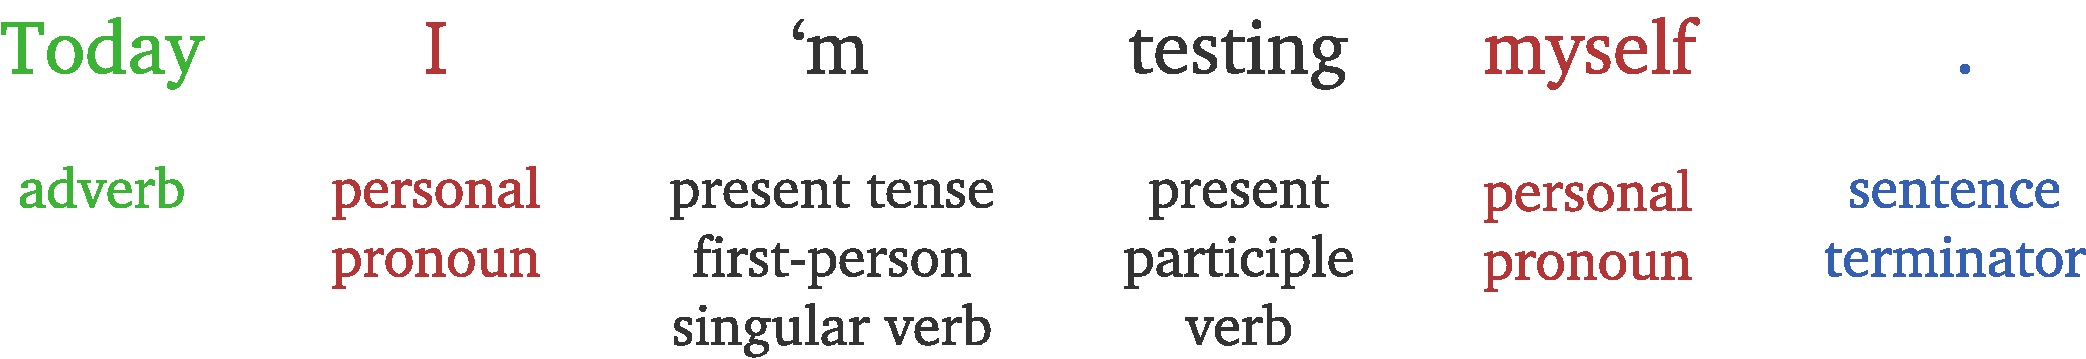
\includegraphics[height=4.5em]{gfx/related-work/posTaggingExample1.pdf}
		\end{center}
	\item \textbf{Named Entity Recognition:}
		Klassifizierung von Tokens in Kategorien wie z.~B. Person, Ort oder Zeitpunkt.
		\[
			({\color{gruen}\underbrace{\text{Today}}_{\text{date}}}, \text{I}, \text{'m}, \text{testing}, \text{myself}, \text{.})
		\]
	\item \textbf{Coreference Resolution:}
		Bestimmung von Token-Äquivalenzklassen, die jeweils auf das selbe Konzept verweisen (insbesondere Pronomina und ihr Antezedens).
		\begin{align*}
			(\text{Today}, \tikzmark{a}\text{\color{rot}I}, \text{'m},
			 \text{testing}, \text{\color{rot}my}\tikzmark{b}\text{\color{rot}self}, \text{.})
			\begin{tikzpicture}[overlay,remember picture]
				\draw[-,rot,shorten >=3pt,shorten <=3pt] (a.center) to[bend right] (b.center);
			\end{tikzpicture}
		\end{align*}
	\item \textbf{Dependency Parsing:}
		Eine auf den POS-Tags aufbauende syntaktische Analyse, welche die grammatikalischen Abhängigkeiten der Token untereinander ausgibt.
		Die Menge dieser Abhängigkeiten bildet einen Baum oder baumähnlichen Graphen, der \textit{Treebank} bzw.\ \textit{Dependency Graph} genannt wird.
		\begin{center}
			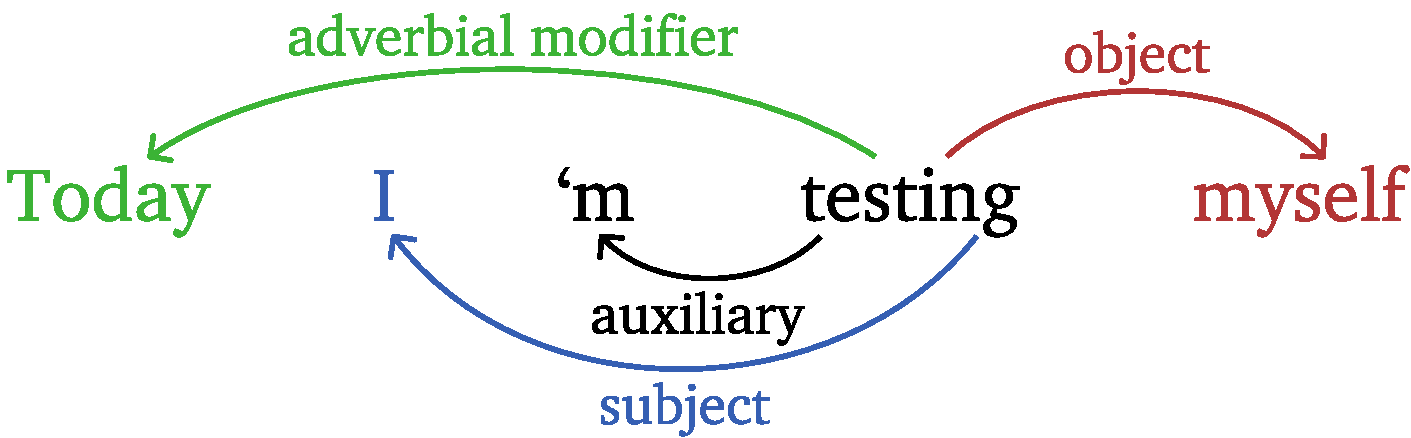
\includegraphics[height=5.5em]{gfx/related-work/depParseExample1.pdf}
		\end{center}
\end{enumerate}

Wie sich erkennen lässt, bauen die Verarbeitungsschritte sukzessive aufeinander auf und bilden eine Art Pipeline.
Dieses Pipeline-Modell findet sich auch in vielen NLP-Werkzeugen wieder.
Ein solches ist z.~B. das quelloffene Stanford~CoreNLP Projekt~\cite{Manning2014}\cite{CoreNLP}, welches u.~a. Module für alle der soeben vorgestellten Verarbeitungsschritte beinhaltet.
Ein alternatives NLP-Toolkit ist Apache~OpenNLP~\cite{OpenNLP};\@
es bietet ähnliche Module wie CoreNLP an.

\section{Wissensgraphkonstruktionsverfahren}%
\label{sec:related:kgc}

Wie in~\ref{sec:related:kr:today} gezeigt, gibt es diverse Ansätze um Graphen aus Daten zu konstruieren.
Da für das Thema dieser Arbeit insbesondere automatisierte Verfahren relevant sind, die mit unstrukurierten Daten, wie z.~B. natürlicher Sprache, umgehen können, werden diese im Folgenden näher beschrieben.

Üblicherweise arbeiten Wissensgraphkonstruktionsverfahren nicht direkt mit den unstrukturierten Eingabedaten, wie z.~B. den Inhalten von E-Mails,
sondern mit einer Knoten- bzw.\ Konzeptmenge und ggf.\ auch einer Kanten- bzw.\ Relationsmenge, die zuvor, z.~B. mittels eines in~\ref{sec:related:nlp} vorgestellten NLP-Verfahrens, aus den Rohdaten extrahiert wurden.
Die Wissensgraphkonstruktion ist somit äquivalent zum Problem der \textit{Link Prediction}, also dem Finden von Relationen zwischen den gegebenen Konzepten.
Die Link Prediction wiederum lässt sich als ein Problem des \textit{Statistical Relational Learnings} (SRL) auffassen.
In der Literatur finden sich im Wesentlichen drei Klassen von SRL-Verfahren~\cite{Nickel2016}, die auf verschiedenen Annahmen über die Korrelation der zu verknüpfenden Informationen basieren:
\begin{enumerate}
	\item \textbf{Latent Feature Models:}
		Alle Relationen werden als bedingt unabhängig angenommen, sofern bestimmte Eigenschaften über Subjekte und Objekte der Relationen gegeben sind.
	\item \textbf{Graph Feature Models:}
		Alle Relationen werden als bedingt unabhängig angenommen, sofern bestimmte Eigenschaften der Struktur des Graphen gegeben sind.
	\item \textbf{Markov Random Fields:}
		Es wird angenommen und erlaubt, dass alle Relationen lokale Abhängigkeiten voneinander haben können.
\end{enumerate}

\paragraph{Latent Feature Models}
Ein Beispiel für ein Latent Feature Modell ist das RESCAL-Verfahren~\cite{Nickel2013}, welches auf Tensorfaktorisierung basiert.
Die Grundidee dabei ist es, allen Entitäten $i$ einen Feature-Vektor $e_i \in \mathbb{R}^H$ zuzuordnen und für alle Relationen $k$ eine Gewichtsmatrix $W_k \in \mathbb{R}^{H \times H}$ zu finden.
Die Konfidenz in die Existenz einer Relation $i \xrightarrow{k} j$ wird durch $e_i^T\ W_k\ e_j$ beschrieben.
Diese Definition ermöglicht eine sehr schnelle Link Prediction, da lediglich ein Vektor-Matrix-Vektor-Produkt berechnet werden muss.
RESCAL liefert gute Ergebnisse, wenn die vorherzusagenden Relationen globale Abhängigkeiten aufweisen.
Lokal stark zusammenhängende Teilgraphen werden allerdings schlecht erkannt, da nur der Feature-Vektor und nicht die Nachbarschaft einer Entität berücksichtigt wird;
ein Beispiel hierfür sind symmetrische Relationen.
\[A \xrightarrow{\text{married to}} B \implies B \xrightarrow{\text{married to}} A\]

\paragraph{Graph Feature Models}
Komplementär zu den Latent Feature Modellen sind die Graph Feature Modelle.
Statt Entitäten in einen Feature-Raum einzubetten, wird hier die Nachbarschaft der Entitäten betrachtet.
Ein Beispiel hierfür ist der \textit{Path Ranking Algorithmus} (PRA)~\cite{Lao2011}. PRA ermittelt Relationen durch zufälliges Durchwandern des Graphen.
Um die Stärken der Latent Feature und Graph Feature Modelle zu kombinieren, wurden Hybrid-Modelle, wie z.~B. das \textit{Additive Relational Effects} (ARE) Verfahren~\cite{Nickel2014}, entwickelt, welches die Konfidenzen von RESCAL und PRA addiert.

\paragraph{Markov Random Fields}
Fundamental verschieden von diesen beiden Verfahren sind \textit{Markov Random Fields} (MRFs).
Hier sind prinzipiell Abhängigkeiten zwischen allen Relationen möglich, was MRFs sehr flexibel macht.
Da dies hinsichtlich der Laufzeit schnell impraktikabel wird, wird das Modell um einen Abhängigkeitsgraphen erweitert, der die Anzahl von betrachteten Abhängigkeiten reduziert.
Der Abhängigkeitsgraph darf dabei nicht mit dem Wissensgraphen verwechselt werden:
Ersterer beschreibt statistische Abhängigkeiten zwischen Klassen von Relationen, während letzterer Abhängigkeiten zwischen spezifischen Fakten beschreibt.
Zur Modellierung von Abhängigkeitsgraphen werden i.~d.~R. Kalküle verwendet, die an eine Prädikatenlogik erster Ordnung angelehnt sind.
Das Finden eines Wissensgraphen ist in diesem Modell äquivalent zum Lösen des MAX-SAT-Problems.
Wählt man ein Kalkül in dem die Atome stetig, also aus $[0, 1]$ statt aus $\{ 0, 1 \}$ sind, und Formeln zudem ausschließlich Disjunktionen und Negationen gemäß Łukasiewicz S-Norm enthalten, erhält man ein sog.\ \textit{Hinge-Loss-MRF}~\cite{Bach2013}\cite{Bach2015}, da die Loss-Funktion der Disjunktion in dieser S-Norm ein Hinge-Loss ist.

Ein konkretes Kalkül, welches sich zur Spezifikation von HL-MRFs eignet, ist die \textit{Probabilistic Soft Logic} (PSL)~\cite{Broecheler2010}\cite{Bach2015}.
MAX-SAT lässt sich für solche HL-MRFs effizient und parallelisierbar mit dem konvexen \textit{Alternating Direction Method of Multipliers} (ADMM) Optimierungsverfahren~\cite{Boyd2011} lösen.
In dessen ursprünglichen Form ist ADMM allerdings ausschließlich für offline Inferenz geeignet;
der Wissensgraph müsste also bei jeder Eingabe neu konstruiert werden.
Um dieses Problem zu lösen, wurde das \textit{Budgeted Online Collective Inference} (BOCI) Verfahren~\cite{Pujara2015} entwickelt.
BOCI nutzt Metadaten, die während der Ausführung von ADMM anfallen, um eine Bewertung für jedes Atom zu berechnen.
Die Bewertung eines Atoms beschreibt, wie groß die erwartete Wertveränderung beim Eintreffen neuer Informationen ist.
Kommen nun neue Informationen an, müssen diese ausschließlich zusammen mit den $m$ höchstbewerteten bereits existierenden Atomen betrachtet werden, die Werte aller anderen Atome werden fixiert.
Je höher das Budget $m$, desto höher ist die Qualität im Vergleich zu einer Neukonstruktion des Graphen.
Es wurde empirisch gezeigt, dass die Inferenzqualität mit BOCI oft nur unwesentlich schlechter ist als bei einer kompletten offline Inferenz.

Mittels ADMM und BOCI lässt sich PSL daher für die online Wissensgraphkonstruktion einsetzen.
Der Vorteil dieses Ansatzes gegenüber eines Latent Feature oder Graph Feature Modells ist, dass sich andere domänenspezifische Expertensysteme leicht in eine PSL Inferenz integrieren lassen.
PSL erlaubt nämlich die Inklusion von benutzerdefinierten Funktionen und Prädikaten.
Diese können benutzt werden, um z.~B. die Levenshtein-Distanz zweier Zeichenketten oder domänenspezifisches Hintergrundwissen, wie Distanz zwischen zwei namentlich genannten Orten, mit in die Entity Resolution einfließen zu lassen.

% !TEX root = ../main.tex
% chktex-file 46
\chapter{Theoretische Grundlagen}%
\label{sec:theory}

In Kapitel~\ref{sec:related} wurde ein Überblick über das Problemumfeld der Wissensgraphkonstruktion gegeben.
Diese Arbeit baut insbesondere auf den bereits kurz vorgestellten Konzeptgraphen, Stanfords~CoreNLP Bibliothek und der PSL auf.
Für die folgenden Kapitel ist ein Grundverständnis dieser drei Themen notwendig.
Sie werden daher in den folgenden Abschnitten näher beschrieben.

\section{Wissensmodellierung mit Konzeptgraphen}%
\label{sec:theory:cg}

John F. Sowas Konzeptgraphen bilden die Basis der Graphontologie dieser Arbeit.
Wie in~\ref{sec:related:kr:history} beschrieben, sind sie ein auf Existenzgraphen basierendes logisches Kalkül.
Die vollständige Konzeptgraphsyntax geht allerdings weit über die Prädikatenlogik hinaus, da auch Modallogik und natürlichsprachliche Konzepte, wie z.~B. Fragen und Betonungen, unterstützt werden.
Da Sowas eigene Beschreibungen diesbezüglich teils etwas unklar sind, werden im folgenden lediglich die sog.~\textit{Conceptual Graphs with Cuts}~\cite{Dau2003} vorgestellt.
Sie sind eine zur Prädikatenlogik erster Ordnung äquivalente, formal spezifizierte Teilmenge der Konzeptgraphen, deren Vollständigkeit und Korrektheit bewiesen ist.

\subsection{Syntax}%
\label{sec:theory:cg:syntax}

In ihrer einfachsten Form lassen sich Konzeptgraphen als Graphen mit drei Arten von Knoten und zwei Arten von Kanten beschreiben.
\begin{itemize}
	\item \textbf{Konzeptknoten (\textit{concepts}):}
		Entsprechen in etwa existenzquantisierten gebundenen Variablen.
		Wie auch in der Prädikatenlogik, haben die Bezeichner von Konzeptknoten keine semantische Relevanz und können frei gewählt werden.
		\begin{align*}
			\vcenter{\hbox{
\includegraphics[height=1.5em]{gfx/theory/conceptNode.pdf}}}
			\quad\Leftrightarrow\quad
			{\color{rot}\exists\ a, b} \numberthis
		\end{align*}
	\item \textbf{Relationsknoten (\textit{conceptual relations}) und Argumentkanten (\textit{arguments}):}
		Relationsknoten entsprechen prädikatenlogischen Atomen.
		Das Symbol innerhalb eines Relationsknoten gibt die Relation des Atoms an.
		Für die Repräsentation der Argumente werden sog.~Argumentkanten zwischen Relationsknoten und Konzeptknoten verwendet.
		Die Position der Argumente bei mehrstelligen Relationen werden durch Nummerierung der Argumentkanten oder bei zweistelligen Relationen durch gerichtete Argumentkanten abgebildet.
		Wenn in einem Graphen mehrere Relationsknoten bzw.\ Atome auftauchen, werden diese als \textit{UND}-verknüpft interpretiert;
		für die Abbildung von \textit{ODER} wird die Negation verwendet.
		\begin{align*}
			\vcenter{\hbox{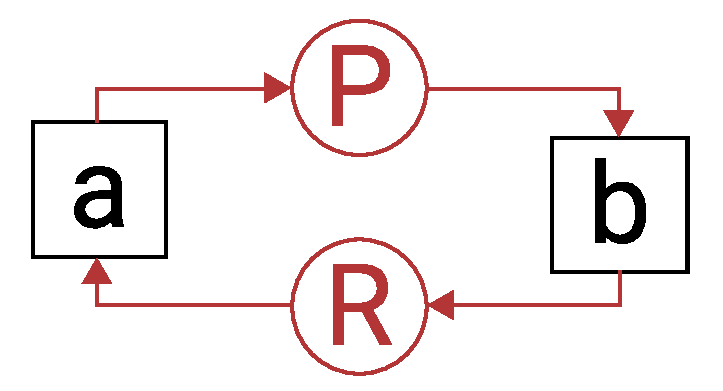
\includegraphics[height=3.75em]{gfx/theory/relationNode.pdf}}}
			\quad\Leftrightarrow\quad
			\exists\ a, b:\ {\color{rot}P(a, b) \land R(b, a)} \numberthis
		\end{align*}
	\item \textbf{Negationskontexte (\textit{negation contexts} oder \textit{cuts}):}
		Für die Negation von Aussagen werden in Konzeptgraphen sog.~Kontexte verwendet.
		Sie lassen sich neben der Negation auch zur Modellierung anderer Zusammenhänge nutzen, diese werden hier allerdings ausgelassen, um den Vergleich mit der Prädikatenlogik zu ermöglichen.
		\begin{align*}
			\vcenter{\hbox{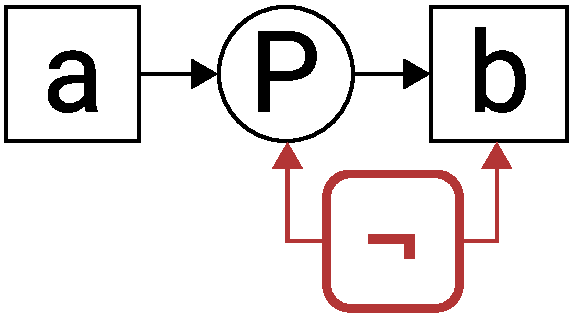
\includegraphics[height=3em]{gfx/theory/negationNode1.pdf}}}
			\quad\Leftrightarrow\quad
			&\exists\ a\ {\color{rot}\lnot\exists}\ b: P(a, b) \numberthis \\
			\quad\Leftrightarrow\quad
			&\exists\ a\ {\color{rot}\forall}\ b: {\color{rot}\lnot} P(a, b)
		\end{align*}
		Die Darstellung von Kontexten mit Knoten und Kanten wird schnell unübersichtlich, daher werden stattdessen Boxen verwendet, die die Kindknoten umschließen.
		\begin{align*}
			\vcenter{\hbox{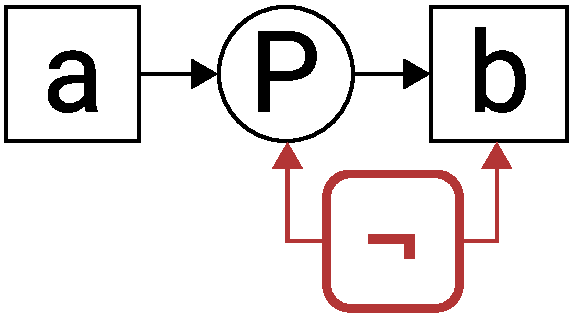
\includegraphics[height=3em]{gfx/theory/negationNode1.pdf}}}
			\quad\Leftrightarrow\quad
			\vcenter{\hbox{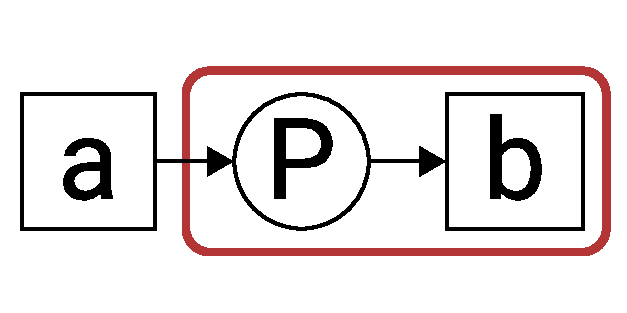
\includegraphics[height=3em]{gfx/theory/negationNode2.pdf}}}
		\end{align*}
		Kontexte können nicht nur Konzeptknoten und Relationsknoten enthalten, sondern auch andere Kontexte.
		Hierbei ist zu beachten, dass alle Knoten und Kontexte höchstens einen Elternkontext haben können;
		die Linien zweier Kontextboxen dürfen sich also nicht schneiden.
		\begin{align*}
			\vcenter{\hbox{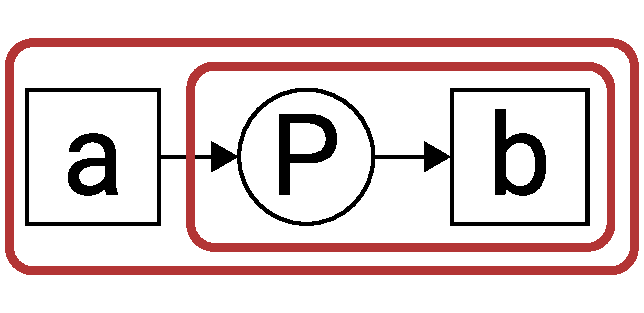
\includegraphics[height=3em]{gfx/theory/negationNode3.pdf}}}
			\quad\Leftrightarrow\quad
			&{\color{rot}\lnot\exists}\ a\ {\color{rot}\lnot\exists}\ b: P(a, b) \numberthis \\
			\quad\Leftrightarrow\quad
			&{\color{rot}\forall}\ a\ \exists\ b: P(a, b)
		\end{align*}
		\begin{align*}
			\vcenter{\hbox{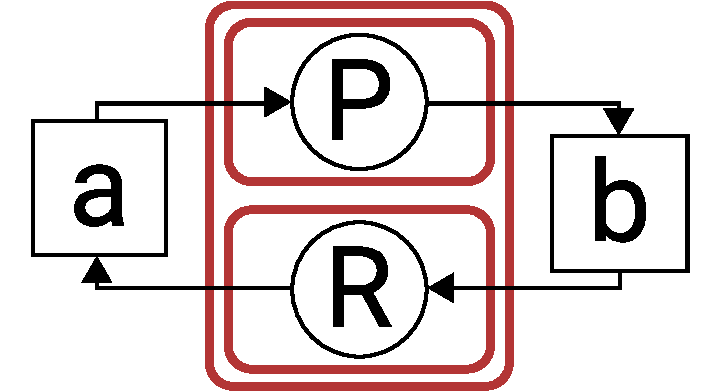
\includegraphics[height=3.75em]{gfx/theory/negationNode4.pdf}}}
			\quad\Leftrightarrow\quad
			&\exists\ a, b: {\color{rot}\lnot}({\color{rot}\lnot} P(a, b) \land {\color{rot}\lnot} R(b, a)) \numberthis \\
			\quad\Leftrightarrow\quad
			&\exists\ a, b: P(a, b)\ {\color{rot}\lor}\ R(b, a)
		\end{align*}
	\item \textbf{Koreferenzkanten (\textit{coreference links}):}
		Entspricht der Äquivalenzrelation.
		\begin{align}
			\vcenter{\hbox{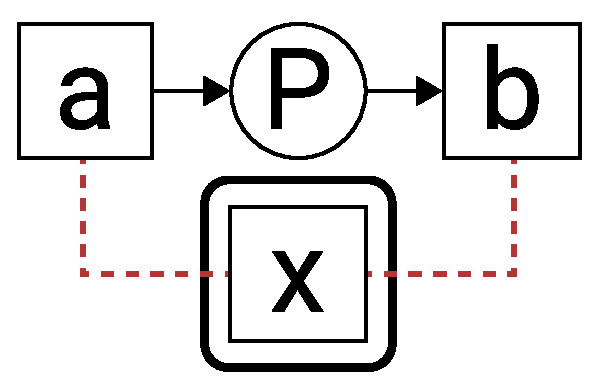
\includegraphics[height=3.75em]{gfx/theory/coreferenceEdge.pdf}}}
			\quad\Leftrightarrow\quad
			&\exists\ a, b: P(a, b) \land \lnot\exists\ x: {\color{rot}a = x \land x = b} \\
			\quad\Leftrightarrow\quad
			&\exists\ a, b: P(a, b) \land {\color{rot}a \neq b} \nonumber
		\end{align}
		Prinzipiell ließe sich die Äquivalenz auch durch Relationsknoten ausdrücken.
		Um syntaktisch zu kennzeichnen, dass es sich nicht um eine beliebige Relation, sondern um eine Äquivalenzrelation handelt, wird dies jedoch i.~d.~R. nicht getan.
		Koreferenzkanten können also als eine Kurzschreibweise verstanden werden, die den Zweck hat die für die Inferenz relevanten Symmetrie-, Transitivitäts- und Reflexivitätseigenschaften zu kennzeichnen.
		\begin{align*}
			\vcenter{\hbox{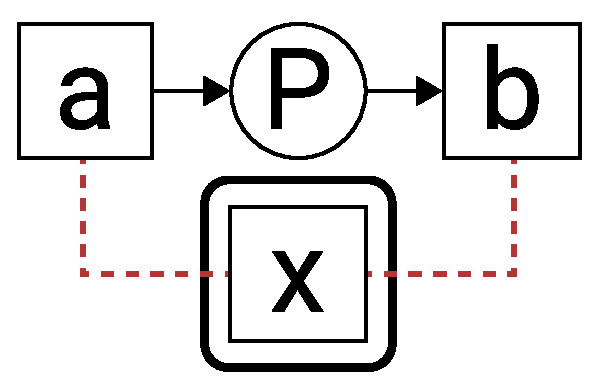
\includegraphics[height=3.75em]{gfx/theory/coreferenceEdge.pdf}}}
			\quad\Leftrightarrow\quad
			\vcenter{\hbox{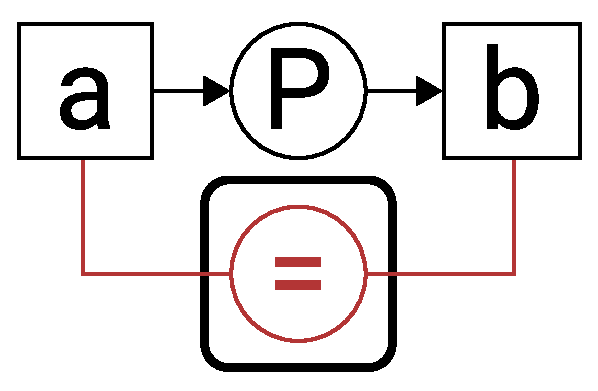
\includegraphics[height=3.75em]{gfx/theory/coreferenceEdgeAlternative.pdf}}}
		\end{align*}
\end{itemize}

\subsection{Dominierende Knoten}%
\label{sec:theory:cg:domnodes}

So wie die Syntaxelemente prädikatenlogischer Ausdrücke nicht beliebig kombiniert werden können, unterliegen auch Konzeptgraphen gewissen Einschränkungen.
Die Einschränkung, dass alle Knoten und Kontexte höchstens einen Elternkontext haben dürfen, wurde bereits erwähnt.
Die zweite wichtige Einschränkung ist das Verbot nicht dominierender Knoten (\textit{dominating nodes}).
Was genau dies bedeutet, wird im Folgenden erläutert. Zuerst müssen Konzeptgraphen jedoch formal spezifiziert werden.
\begin{align*}
	G :=\ &(V, E) \text{, mit globalem Kontext } \top \in V \\
	concept(v) :\Leftrightarrow\ &\text{$v \in V$ ist ein Konzeptknoten} \\
	relation(v) :\Leftrightarrow\ &\text{$v \in V$ ist ein Relationsknoten} \\
	context(v) :\Leftrightarrow\ &\text{$v \in V$ ist ein Kontext, es gilt $context(\top)$} \\
	neg(v) :\Leftrightarrow\ &\text{$v \in V$ ist ein Negationskontext} \displaybreak[0]\\
	nest(c, v) :\Leftrightarrow\ &context(c) \land (c, v) \in E \\
	coref(v_1, v_2) :\Leftrightarrow\ &concept(v_1) \land concept(v_2) \land (v_1, v_2) \in E \\
	arg(r, v) :\Leftrightarrow\ &relation(r) \land concept(v) \land ((r, v) \in E \lor (v, r) \in E) \\ % chktex 35
	E \supseteq\ &\{ (\top, v): v \in V \land \lnot\exists\ c \in V: nest(c, v) \} \displaybreak[0]\\
	a \leq b :\Leftrightarrow\ & (\exists\ x \in V: a \leq x \land x \leq b) \numberthis \\
	& \lor nest(b, a) \lor (\exists\ c \in V: nest(c, a) \land nest(c, b))
\end{align*}
Um die nachfolgenden Definitionen einfacher zu machen, wird der globale Kontext $\top$ eingeführt, der, in Anlehnung an Peirce, \textit{sheet of assertion} genannt wird.
$\top$ enthält alle Knoten, die keinen explizit dargestellten Elternkontext haben.
Die Kontextbox von $\top$ umschließt also den gesamten Konzeptgraphen.
$\leq$ ist eine Quasiordnung und bildet die \textit{enthalten-in}-Relation zwischen Knoten ab, d.~h.\ $a \leq b$ gdw.\ $a$ innerhalb der Box des Elternkontextes von $b$ liegt.
Das größte Element gemäß $\leq$ ist also immer $\top$.
\begin{figure}[h]
	\centering
	\[\vcenter{\hbox{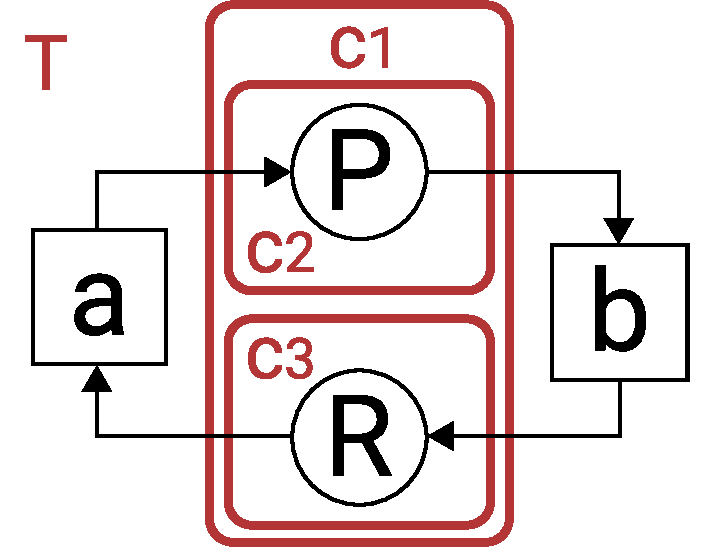
\includegraphics[height=5.25em]{gfx/theory/contextTreeExample1.pdf}}}
	\qquad
	\vcenter{\hbox{
		\begin{tikzpicture}[
			grow=down,
			sloped,
			level distance=2em,
			sibling distance=3em,
			edge from parent/.style={draw=black!70,latex-}]
			\node {\color{rot}$\top$}
				child {
					node (a) {$a$}
				}
				child {
					node (c1) {\color{rot}$c_1$}
						child {
							node (c2) {\color{rot}$c_2$}
								child {
									node {$P$}
								}
						}
						child {
							node (c3) {\color{rot}$c_3$}
								child {
									node {$R$}
								}
						}
				}
				child {
					node (b) {$b$}
				};
				\draw[latex-latex] (a) -- (c1);
				\draw[latex-latex] (c1) -- (b);
				\draw[latex-latex] (c2) -- (c3);
		\end{tikzpicture}
	}}\]
	\caption{Zusammenhang zwischen Kontexten und der $\leq$-Ordnung. Die Existenz eines Pfades von $x$ nach $y$ im obigen baumartigen Graphen, entspricht $x \leq y$.}\label{fig:theory:kgorder}
\end{figure}

Auf Basis von $\leq$ lässt sich nun das Konzept dominierender Knoten definieren.
\begin{align*}
	dom(G) :\Leftrightarrow\ & \forall\ r, v \in V: arg(r, v) \rightarrow r \leq v \numberthis \\ % chktex 35
	& \land \forall\ v_1, v_2 \in V: coref(v_1, v_2) \rightarrow (v_1 \leq v_2 \lor v_2 \leq v_1)
\end{align*}
Für jeden Konzeptgraphen $G$ muss $dom(G)$ gelten.
Eine Intuition für diese Einschränkung ist, dass es nicht sinnvoll ist die Existenz eines Atoms auszudrücken, welches durch nicht existente Variablen parametrisiert ist.
Eine detaillierte Untersuchung des Zwecks dominierender Knoten und eine Beschreibung der entstehenden Probleme, wenn auf die Notwendigkeit dominierender Knoten verzichtet wird, findet sich in~\cite[Abschnitt~14.3]{Dau2003}.
\begin{figure}[h]
	\begin{align*}
		\vcenter{\hbox{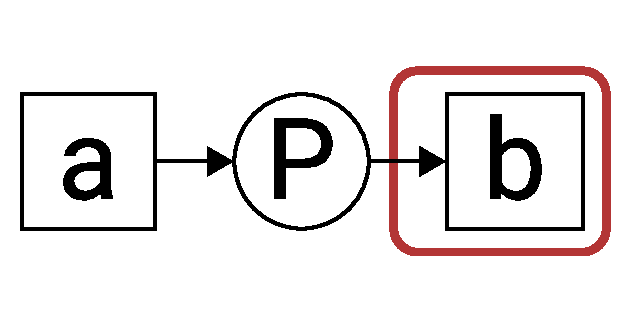
\includegraphics[height=3em]{gfx/theory/dominatingNodeViolation1.pdf}}}
		\quad
		&\text{\color{rot}$\lightning\ \lnot dom(G)$, da $arg(P, b) \land \lnot (P \leq b)$.} \\ % chktex 35
		\vcenter{\hbox{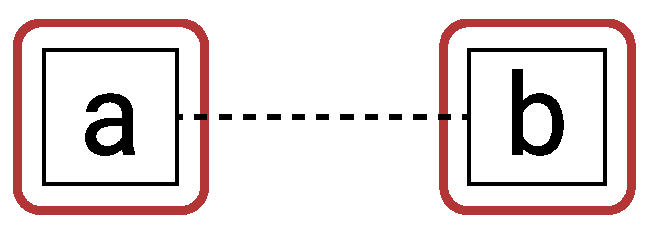
\includegraphics[height=2.25em]{gfx/theory/dominatingNodeViolation2.pdf}}}
		\quad
		&\text{\color{rot}$\lightning\ \lnot dom(G)$, da $coref(a, b) \land \lnot (a \leq b \lor b \leq a)$.}
	\end{align*}
	\caption{Beispiele für fehlerhafte Konzeptgraphen ohne dominierende Knoten.}\label{fig:theory:invalidkg}
\end{figure}

\section{Stanford CoreNLP}%
\label{sec:theory:nlp}

Um natürlichsprachliche Daten in einen Konzeptgraphen zu transformieren, ist im ersten Schritt eine Sprachanalyse notwendig.
Hierfür wurde die Stanford CoreNLP~\cite{CoreNLP} und die Apache OpenNLP~\cite{OpenNLP} Bibliothek in Erwägung gezogen, da beide häufig genutzt, aktiv weiterentwickelt, frei verfügbar und JVM-basiert sind.
Die JVM-Integration ist wichtig, um mit anderen verwendeten Bibliotheken kompatibel zu sein;
mehr hierzu in Abschnitt~\ref{sec:text2kg:implementation}.
Für die Implementation wurde schließlich CoreNLP gewählt, da es mit den mitgelieferten Modellen häufig bessere Ergebnisse als OpenNLP liefert.
Da beide Bibliotheken bzgl.\ ihrer Funktionalität allerdings recht ähnlich sind, kann die NLP Komponente als substituierbar angesehen werden.
Ein Wechsel von CoreNLP auf OpenNLP wäre mit relativ geringem Aufwand möglich.

Im Folgenden wird nun die grundlegende Architektur von CorenNLP beschrieben.
CoreNLP verwendet das in~\ref{sec:related:nlp} vorgestellte Pipeline-Modell.
Die verschiedenen Verarbeitungsstufen der Pipeline werden Annotatoren genannt.
Da die genaue Funktionsweise der Annotatoren ist für diese Arbeit weniger relevant, wichtiger ist ein Überblick über die Art der Ergebnisse, die die Annotatoren liefern.

\paragraph{Tokenization und Lemmatization}
Liefern, wie erwartet, eine Liste von Token bzw.\ eine Liste der Lemmata der Token.
Es werden neben Englisch zahlreiche andere Sprachen und ein Großteil des Unicode Zeichensatzes unterstützt.
Der Tokenizer verwendet zum Finden der Tokens intern einen deterministischen endlichen Automaten.

\paragraph{POS-Tagging}
Ordnet jedem Token eine Wortart und Flexion (POS-Tag) zu.
Die Menge der möglichen POS-Tags wurde aus dem \textit{Penn Treebank Tag Set}~\cite{PennTags} übernommen.
Für das Finden der Tags benutzt CoreNLP sog.\ \textit{Cyclic Dependency Networks}~\cite{Toutanova2003}, eine Erweiterung bayesscher Netze, in denen zyklische Abhängigkeiten erlaubt sind.

\paragraph{Named Entity Recognition (NER)}
Findet sog.\ Entitäten.
CoreNLP benutzt hierfür eine Menge von Entitätsklassen, die sich in drei Kategorien von Klassen unterteilen lässt:
\begin{enumerate}
	\item \textbf{Benannte Entitäten:}
		Person, Ort, Organisation und Sonstige.
		Diese Entitätsklassen werden mittels \textit{Conditional Random Fields}~\cite{Finkel2005}, einer Variante von \textit{Markov Random Fields} (siehe~\ref{sec:theory:psl:mrf}), erkannt.
	\item \textbf{Numerische Entitäten:}
		Geldbetrag, Zahl, Ordinalzahl und Prozentzahl.
		Hierfür wird ein regelbasiertes System verwendet.
		Die so erkannten Token werden zudem normalisiert, um eine leichtere Weiterverarbeitung zu ermöglichen.
	\item \textbf{Temporale Entitäten:}
		Datum, Uhrzeit, Dauer und Menge von Zeitpunkten.
		Diese Klassen werden ebenfalls mit einem regelbasierten System erkannt.
		Mittels SUTime~\cite{Chang2012} werden die erkannten Token anschließend normalisiert und relative Zeitangaben in absolute Zeitpunkte aufgelöst, sofern ein Referenzzeitpunkt gegeben ist.
		Für die Normalisierung wird das TimeML TIMEX3-Format~\cite{TIMEX3} benutzt, mit dem sich auch komplexe Zeitangaben, wie \textit{``twice a week''} (\texttt{type=''set'' value=''P1W'' freq=''2X''}), formal ausdrücken lassen.
\end{enumerate}

\paragraph{Coreference Resolution}
Ermittelt Äquivalenzklassen von Token, die auf das selbe Konzept bzw.\ die selbe Entität verweisen.
CoreNLP stellt hierfür drei verschiedene Systeme bereit:
Ein schnelles, regelbasiertes, deterministisches System, ein etwas langsameres statistisches System und zuletzt ein langsames System, das auf neuronalen Netzen basiert.
Die langsameren Systeme liefern im Schnitt bessere Ergebnisse.

\paragraph{Dependency Parsing}
Dieser Annotator ermittelt die grammatikalischen Beziehungen zwischen Worten.
Das Ergebnis ist ein sog.\ Abhängigkeitsgraph (\textit{Dependency Graph}), in dem die Knoten Token und die Kanten Beziehungen repräsentieren.
CoreNLP verwendet für die Kantentypen \textit{Universal Dependencies Version 2} (UD v2)~\cite{UDv2}, eine Menge von 37 Arten grammatikalischer Beziehungen, die für eine vielzahl natürlicher Sprachen nutzbar ist.
Die Struktur der zurückgegebenen Abhängigkeitsgraphen, basiert auf einem ``\textit{{\color{blau}head}-{\color{rot}modifier}}''-Pattern;
d.~h.\ dass, ausgehend von einem \textit{\color{blau}head}-Token, Kanten zu \textit{\color{rot}modifier}-Token gehen, die die Bedeutug des \textit{\color{blau}heads} verändern.
\[
	\text{\color{rot}Peter's} \xleftarrow{\text{possessive nominal modifier}}
	\text{\color{blau}ball}
	\xrightarrow{\text{adjectival modifier}} \text{\color{rot}red}
\]
Der CoreNLP Dependency Parser nutzt ein sog.\ \textit{Transition-based Parsing}~\cite{Nivre2004}, bei dem alle Token der Reihe nach aus einem Buffer auf einen Stack von aktuell betrachteten Token gelegt werden.
Ein Klassifikator (im Falle von CoreNLP ist dies ein neuronales Netz) wählt dabei in jedem Schritt einen von drei Zustandsübergängen:
\begin{enumerate}
	\item \textbf{LEFT-ARC:}
		Fügt eine Abhängigkeitskante $(i, j)$ vom ersten Token $i$ des Stacks zum zweiten Token $j$ des Stacks ein und entfernt dann $j$ vom Stack.
	\item \textbf{RIGHT-ARC:}
		Fügt eine Abhängigkeitskante $(j, i)$ vom zweiten Token $j$ des Stacks zum ersten Token $i$ des Stacks ein und entfernt dann $i$ vom Stack.
	\item \textbf{SHIFT:}
		Verschiebt das erste Token des Buffers auf den Stack.
\end{enumerate}
Diese drei Zustandsübergänge werden so lange angewandt, bis der Buffer leer ist.
Durch die richtige Kombination von Übergängen lässt sich jeder beliebige Abhängigkeitsgraph beschreiben.

\section{Modellierung von HL-MRFs mit PSL}%
\label{sec:theory:psl}

In~\ref{sec:theory:cg} wurde beschrieben, wie komplexes Wissen durch Konzeptgraphen repräsentiert werden kann;
in~\ref{sec:theory:nlp} wurde beschrieben, wie der Inhalt natürlichsprachlicher Texte extrahiert und durch eine Menge von Abhängigkeiten repräsentiert werden kann.
Dieser Abschnitt beschreibt nun, wie aus einer Menge gegebenener Abhängigkeiten und Fakten neue Abhängigkeiten und Fakten inferiert werden können.
Konkrekt werden hierfür \textit{Hinge-Loss Markov Random Fields} (HL-MRFs) und die \textit{Probabilistic Soft Logic} (PSL) vorgestellt.

\subsection{Markov Random Fields}%
\label{sec:theory:psl:mrf}

MRFs sind, so wie auch bayessche Netze, eine Klasse von \textit{Probabilistischen Graphischen Modellen} (PGM);
d.~h.\ sie sind Graphen, deren Knoten als Zufallsvariablen und deren Kanten als stochastische Abhängigkeiten interpretiert werden.
Im Gegensatz zu bayesschen Netzen, sind die Kanten in MRFs allerdings ungerichtet, es sind also zyklische Abhängigkeiten erlaubt.
Formal beschreibt ein MRF $G$ die multivariate Verteilung $P$ eines Zufallsvektors $X$ gemäß einer Potentialfunktion $\Phi$:
\begin{align*}
	X :=&\ (X_1, \dots, X_n) = \text{Zufallsvektor} \\
	\mathcal{X} :=&\ \text{Menge aller möglichen Werte $(x_1, \dots, x_n)$ von $X$} \\
	G :=&\ (X, E) \\
	\mathcal{C} :=&\ \{ c_1, \dots, c_m \} = \text{Menge der maximalen Cliquen in $G$} \displaybreak[0]\\ % chktex 21
	X_c :=&\ \text{Vektor der Zufallsvariablen in der Clique $c \in \mathcal{C}$} \\
	\Phi_c(x_c) :=&\ \text{Cliquenpotential $\in \mathbb{R}^{+}_0$ der Werte $x_c$ von $X_c$} \\
	P(X = x) =&\ \frac{1}{Z} \prod_{i = 1}^{m} \Phi_{c_i}(x_{c_i}) \text{, mit Normalisierkonst. } Z := \sum_{x \in \mathcal{X}} \prod_{i = 1}^{m} \Phi_{c_i}(x_{c_i}) \numberthis
\end{align*}
Für MRFs gelten drei wichtige Eigenschaften bzgl.\ der Unabhängigkeit der Zufallsvariablen in $X$:
\begin{enumerate}
	\item \textbf{Globale Markov-Eigenschaft:}
		\[
			\forall X_A, X_B, X_S \subseteq X: sep_{X_A, X_B}(X_S) \rightarrow (X_A \perp X_B \mid X_S)
		\]
		Alle Paare $(X_A, X_B)$ von Teilmengen von $X$ sind bedingt unabhängig, sofern die Werte einer separierenden Teilmenge $X_S $ gegeben sind.
		$X_S$ ist separierend ($\Leftrightarrow sep_{X_A, X_B}(X_S)$), wenn alle Pfade von $a \in X_A$ nach $b \in X_B$ einen Knoten $s \in X_S$ enthalten.
	\item \textbf{Lokale Markov-Eigenschaft:}
		\[
			\forall X_i \in X: X_i \perp (X \setminus \Gamma(X_i) \setminus \{X_i\}) \mid \Gamma(X_i)
		\]
		Eine direkte Konsequenz der globalen Markov-Eigenschaft ist die lokale Markov-Eigenschaft.
		Jede Variable $X_i$ ist bedingt unabhängig von ihren nicht benachbarten Variablen, sofern ihre Nachbarschaft $\Gamma(X_i)$ gegeben ist.
	\item \textbf{Paarweise Markov-Eigenschaft:}
		\[
			\forall X_i, X_j \in X: \{X_i, X_j \} \notin E \rightarrow (X_i \perp X_j \mid X \setminus \{ X_i, X_j \})
		\]
		Aus der lokalen Markov-Eigenschaft folgt, dass jedes nicht adjazente Variablenpaar $(X_i, X_j)$ bedingt unabhängig voneinander ist, sofern alle anderen Variablen gegeben sind.
\end{enumerate}

\paragraph{Beispiel}
Die obigen Definitionen sind bislang noch recht abstrakt.
Ein exemplarisches praktisches Einsatzgebiet von MRFs ist das Lösen von SAT-Problemen.
Gegeben sei die SAT-Instanz ${\color{rot}(\lnot A \lor B \lor C)} \land {\color{blau}(\lnot C \lor \lnot D)}$.
MRFs können benutzt werden, um dieses Problem zu modellieren und eine erfüllende Belegung zu finden.\\
\begin{tabular}{m{0.25\textwidth} m{0.75\textwidth}}
	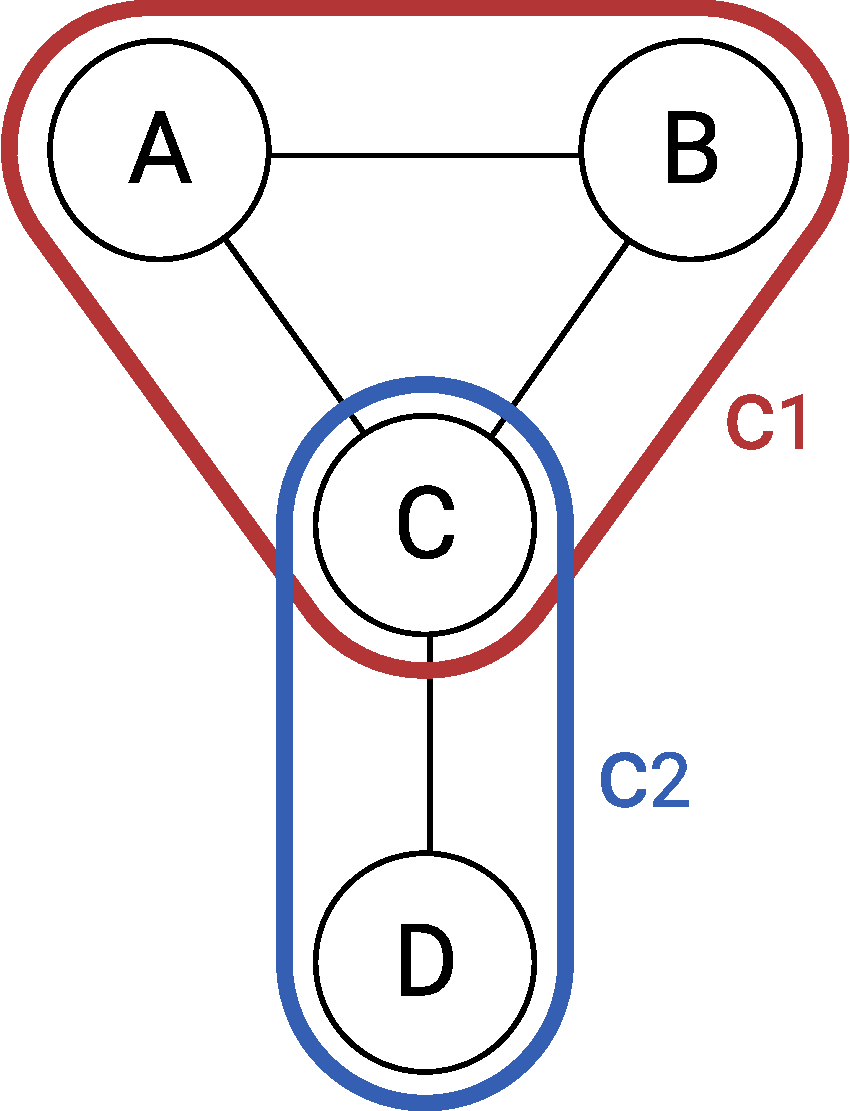
\includegraphics[width=0.23\textwidth]{gfx/theory/mrfExample1.pdf}
	&
	{\begin{align*}
		X :=&\ (A, B, C, D) \text{, mit } Bild(X) = {\{0, 1\}}^4 \\
		\mathcal{C} :=&\ \{{\color{rot}\underbrace{\{ A, B, C \}}_{c_1}}, {\color{blau}\underbrace{\{ C, D \}}_{c_2}}\} \\ % chktex 21
		{\color{rot}\Phi_{c_1}}(a, b, c) :=&\ \min\{ 1 - a + b + c, 1 \} \\ % chktex 21
		{\color{blau}\Phi_{c_2}}(c, d) :=&\ \min\{ 2 - c - d, 1 \} \\ % chktex 21
		P(X = (a, b, c, d)) :=&\ \frac{1}{Z} {\color{rot}\Phi_{c_1}}(a, b, c)\ {\color{blau}\Phi_{c_2}}(c, d)
	\end{align*}}
\end{tabular}\\
Eine Clique repräsentiert in diesem MRF eine Disjunktionsklausel und das Cliquenpotential gibt an, ob eine gegebene Belegung die Klausel erfüllt.
Gemäß dieser Definition, lässt sich die Erfüllbarkeit durch $\max_{x} P(X = x) > 0$ ausdrücken, d.~h.\ die Formel ist erfüllbar, gdw.\ es eine Variablenbelegung mit Eintrittswahrscheinlichkeit~$> 0$ gibt.
Die Normalisierungskonstante $Z$ hat auf das Ergebnis keinen Einfluss und kann daher ignoriert werden.

\paragraph{Das MRF-Inferenzproblem}
Da sich SAT, wie soeben exemplarisch gezeigt, auf MRFs reduzieren lässt, ist das Inferenzproblem, d.~h.\ das Finden einer maximal wahrscheinlichen Belegung der Zufallsvariablen, ein NP-schweres Problem.
Allgemeine, exakte und effiziente Lösungsalgorithmen existieren daher nicht.
Durch Einschränken der Struktur von $G$ und $\Phi$, oder durch das erlauben von Approximationen, lassen sich MRF-Inferenzen jedoch deutlich effizienter finden.
Wenn z.~B. $G$ ein Baum ist, kann mit dem \textit{Belief Propagation} Algorithmus eine exakte Lösung in polynomieller Zeit gefunden werden.

\subsection{Hinge-Loss MRFs}%
\label{sec:theory:psl:hlmrf}

Eine Unterart von MRFs, sind die sog.\ Hinge-Loss MRFs.
Sie sind so strukturiert, dass sich das Inferenzproblem effizient und exakt durch konvexe Optimierungsverfahren lösen lässt.
Es gibt drei wesentliche Unterschiede zu allgemeinen MRFs:
\begin{enumerate}
	\item
		Die Bedeutung von Zufallsvariablen und Kanten zwischen Zufallsvariablen ist klar definiert, da $\Phi$ nicht mehr frei wählbar ist.
		Ähnlich zum Beispiel aus~\ref{sec:theory:psl:mrf}, repräsentieren Zufallsvariablen aussagenlogische Variablen und Cliquen Disjunktionsklauseln.
	\item
		Für den Zufallsvektor $X$ muss $Bild(X) = {[0, 1]}^n$ gelten.
		Diese Einschränkung besteht, da jede HL-MRF-Zufallsvariable als die Wahrscheinlichkeit, dass eine aussagenlogische Variable wahr ist, interpretiert wird.
	\item
		Die Definition der Verteilung $P$ ist etwas anders:
		\begin{align*}
			P(X = x) :=&\ \frac{1}{Z} \prod_{i = 1}^{m} e^{w_i\,\Phi_i(x)} \propto \exp\left(\sum_{i=1}^{m} w_i\,\Phi_i(x)\right) = \exp\left(w\,{\Phi(x)}^\top\right) \numberthis \\
			w :=&\ (w_1, \dots, w_m) \in \mathbb{R}^m,\ \Phi := (\Phi_1, \dots, \Phi_m)
		\end{align*}
		Auf die Cliquenpotentiale $\Phi_i$ wird nun die Exponentialfunktion angewandt, zudem erhalten alle Cliquen bzw.\ Klauseln $c_i$ ein Gewicht $w_i$.
		Das Inferenzproblem $\arg\max_{x} P(X = x)$ ist somit äquivalent zu $\arg\max_{x} w\,{\Phi(x)}^\top$.
\end{enumerate}

\paragraph{KNF-Formel Interpretation}
Aufgrund der Einschränkung von HL-MRFs auf aussagenlogische Ausdrücke, wird im Folgenden die Graphterminologie fallen gelassen und stattdessen die entsprechende aussagen\-logische Terminologie verwendet.
Ein HL-MRF wird nun als Repräsentation einer KNF-Formel $C_1 \land \dots \land C_m$ interpretiert.
Jede Disjunktionsklausel $C_j \in C$ wird durch eine Menge von Variablenindizes positiver Atome $I^{+}_j \subseteq \{1,\dots,n\}$ und eine Menge von Variablenindizes negativer Atome $I^{-}_j \subseteq \{1,\dots,n\}$ beschrieben.
\[
	C_j \cong \left(\bigvee_{i \in I^{+}_j} X_i\right) \lor \left(\bigvee_{i \in I^{-}_j} \lnot X_i\right)
\]

\paragraph{Łukasiewicz Logik}
Da die Variablen der KNF-Formel, gemäß obiger Definition, Werte~$\in [0, 1]$ annehmen können, ist nun noch unklar, wie die Operatoren $\land$, $\lor$ und $\lnot$ funktionieren sollen.
HL-MRFs benutzen hierfür die sog.\ Łukasiewicz Logik aus der Klasse der T-Norm Fuzzy Logiken;
sie ist eine Erweiterung der booleschen Logik, d.~h.\ die Łukasiewicz Operatoren verhalten sich für die Extrema $0$ und $1$ so, wie die booleschen Operatoren, sind aber ebenfalls für alle dazwischen liegenden Eingabewerte definiert.
\begin{align}
	x_1 \land x_2 :=&\ \max\{ x_1 + x_2 - 1, 0 \} \\ % chktex 21
	x_1 \lor x_2 :=&\ \min\{ x_1 + x_2, 1 \} \\ % chktex 21
	\lnot x :=&\ 1 - x
\end{align}
\begin{figure}[h]
	\centering
	\begin{tikzpicture}
		\begin{axis}[
			title={$\land$},
			xlabel=$x_1$,
			ylabel=$x_2$,
			width=0.35\textwidth,
			colormap = {bluered}{color(0cm) = (blau); color(1cm) = (rot)}
		]
			\addplot3[
				mesh,
				samples=12,
				domain=0:1,
				domain y=0:1
			]{max(x + y - 1, 0)};
		\end{axis}
	\end{tikzpicture}
	\begin{tikzpicture}
		\begin{axis}[
			title={$\lor$},
			xlabel=$x_1$,
			ylabel=$x_2$,
			width=0.35\textwidth,
			colormap = {bluered}{color(0cm) = (blau); color(1cm) = (rot)}
		]
			\addplot3[
				mesh,
				samples=12,
				domain=0:1,
				domain y=0:1
			]{min(x + y, 1)};
		\end{axis}
	\end{tikzpicture}
	\begin{tikzpicture}
		\begin{axis}[
			title={$\lnot$},
			xlabel=$x$,
			width=0.35\textwidth,
			colormap = {bluered}{color(0cm) = (blau); color(1cm) = (rot)}
		]
			\addplot[
				surf,
				domain=0:1
			]{1 - x};
		\end{axis}
	\end{tikzpicture}
	\caption{Visualisierung der Łukasiewicz Operatoren $\land$, $\lor$ und $\lnot$.}\label{fig:theory:luklogic}
\end{figure}

Mittels der Łukasiewicz Logik können Disjuktionsklauseln $C_j \in C$ für eine gegebene Variablenbelegung $x$ nun Wahrheitswerte~$\in [0, 1]$ zugeordnet werden.
Dieser Wahrheitswert wird als Klauselpotential $\Phi_j(x)$ verwendet.
Das HL-MRF-Inferenzproblem für KNF-Formeln in Łukasiewicz Logik ist demnach
\begin{alignat*}{3}
	\operatorname*{arg\,max}_{x \in {[0, 1]}^n}& \sum_{C_j \in C} w_j &&\Phi_j(x) \\ % chktex 35
	= \operatorname*{arg\,max}_{x \in {[0, 1]}^n}& \sum_{C_j \in C} w_j &&\left(\left(\bigvee_{i \in I^{+}_j} x_i\right) \lor \left(\bigvee_{i \in I^{-}_j} \lnot x_i\right)\right) \displaybreak[0]\\ % chktex 35
	= \operatorname*{arg\,max}_{x \in {[0, 1]}^n}& \sum_{C_j \in C} w_j \min &&\left\{ \left(\sum_{i \in I^{+}_j} x_i\right) + \left(\sum_{i \in I^{-}_j} (1 - x_i)\right), 1 \right\} \numberthis % chktex 21, chktex 35
\end{alignat*}

Statt die Summe der Wahrheitswerte $\Phi_j(x)$ zu maximieren, kann alternativ auch die Summe der Distanzen zur Erfüllung $\ell_j(x)$, genannt \textit{distance to satisfaction}, minimiert werden;
es gilt $\ell_j(x) = 1 - \Phi_j(x)$.
Gemäß dieser Interpretation ist ein HL-MRF somit eine Menge von gewichteten Constraints $\ell_j(x) \leq 0$, für die eine Lösung mit möglichst wenigen Verletzungen gesucht wird.
Das Inferenzproblem ist also
\begin{align*}
	\operatorname*{arg\,min}_{x \in {[0, 1]}^n}& \sum_{C_j \in C} w_j \max \{ \ell_j(x), 0 \} \displaybreak[0]\\ % chktex 35
	= \operatorname*{arg\,min}_{x \in {[0, 1]}^n}& \sum_{C_j \in C} w_j \max \left\{ 1 - \left(\sum_{i \in I^{+}_j} x_i\right) - \left(\sum_{i \in I^{-}_j} (1 - x_i)\right), 0 \right\} \numberthis % chktex 21, chktex 35
\end{align*}

\begin{figure}[h]
	\centering
	\begin{tikzpicture}
		\begin{axis}[
			xlabel=$x_1$,
			ylabel=$x_2$,
			y dir=reverse,
			width=0.45\textwidth,
			colormap = {bluered}{color(0cm) = (blau); color(1cm) = (rot)}
		]
			\addplot3[
				mesh,
				samples=20,
				domain=0:1,
				domain y=0:1
			]{max(1 - x - y, 0)};
		\end{axis}
	\end{tikzpicture}
	\caption{Visualisierung der Loss-Funktion $\ell_j(x_1, x_2)$ für $C_j \cong X_1 \lor X_2$}\label{fig:theory:hingeloss}
\end{figure}
Wie Abb.~\ref{fig:theory:hingeloss} für den zwei-elementigen Klauselfall veranschaulicht, handelt es sich bei $\ell$ um eine Hinge-Loss Funktion.
Hierher rührt die Bezeichnung Hinge-Loss MRF.\@

\paragraph{MAX-SAT Äquivalenz}
In~\ref{sec:theory:psl:mrf} wurden MRFs anhand des Beispiels der SAT-Instanz ${\color{rot}(\lnot A \lor B \lor C)} \land {\color{blau}(\lnot C \lor \lnot D)}$ veranschaulicht.
Diese KNF-Formel hat folgendes Inferenzproblem, wenn sie als HL-MRF repräsentiert wird:
\[
	\operatorname*{arg\,min}_{(a, b, c, d) \in {[0, 1]}^4} {\color{rot}w_1 \max\{a - b - c, 0\}} + {\color{blau}w_2 \max\{c + d - 1, 0\}} % chktex 21, chktex 35
\]
Da in der Verteilung $P$ von HL-MRFs die Exponentialfunktion auf die Potentiale angewandt wird, bewirkt eine unerfüllte Klausel mit $\Phi_j(x) = 0$ nicht, dass $P(X = x) = 0$.
Stattdessen ist $P(X = x)$ proportional zu der Summe der Wahrheitswerte der Klauseln.
Die HL-MRF-Inferenz beschreibt also nicht SAT, sondern eine Fuzzy-Logik-Entsprechung von MAX-SAT.\@
Ein wichtiger Unterschied zum booleschen MAX-SAT ist, dass Klauseln gewichtet sind;
das Erfüllen einer Klausel mit hohem Gewicht kann das Nicht-Erfüllen mehrerer anderer Klauseln mit niedrigem Gewicht ausgleichen.

\subsection{Probabilistic Soft Logic}%
\label{sec:theory:psl:psl}

Wie soeben beschrieben, sind HL-MRFs ein flexibles Werkzeug, um Probleme, die sich durch MAX-SAT ausdrücken lassen, zu lösen.
Der Schritt von einem konkreten domänenspezifischen Problem in eine Menge von Klauseln $C$ und einen Gewichtsvektor $w$ ist bislang allerdings noch unklar.
An dieser Stelle setzt die \textit{Probabilistic Soft Logic} (PSL) an.
PSL ist eine formale Sprache, um mit einer intuitiven Syntax Klassen von HL-MRFs zu beschreiben.

\subsubsection{Syntax}
Die Syntax von PSL ist an die Prädikatenlogik angelehnt und besteht aus sieben Arten von Elementen:
\begin{enumerate}
	\item \textbf{Konstanten:}
		Repräsentieren konstante Werte, wie z.~B. Strings oder Zahlen.
		Werden für domänenspezifische Daten, wie z.~B. Namen benutzt. \\
		\centerline{\texttt{''Alice'', 32}}
	\item \textbf{Variablen:}
		Werden während einer Inferenz mit Konstanten belegt.
		PSL Variablen sind nicht zu verwechseln mit den Zufallsvariablen in MRFs. \\
		\centerline{\texttt{x, y, z}}
	\item \textbf{Terme:}
		Ein Term ist entweder eine Konstante oder eine Variable.
	\item \textbf{Prädikate:}
		Entsprechen in etwa den prädikatenlogischen Prädikaten.
		Jedes PSL Prädikat hat einen eindeutigen Bezeichner und eine Typsignatur beliebiger Arität.
		Prädikate sind über Konstanten definiert, die Signatur ist daher über den Konstantentypen definiert. \\
		\centerline{\texttt{Person/1: UUID, Name/2: UUID $\times$ String, Age/2: UUID $\times$ Integer}}
	\item \textbf{Atome:}
		Ein Atom ist ein Prädikat der Arität $n$, kombiniert mit einem $n$-Tupel von Termen.
		Das Term-Tupel enthält die Argumente des Prädikates.
		Wenn alle Argumente Konstanten sind, spricht man von einem Grundatom (\textit{ground atom}). \\
		\centerline{\texttt{Person(x), Name(x, ''Alice''), Age(x, 32)}} % chktex 32, chktex 36
	\item \textbf{Literale:}
		Ein Literal ist entweder ein Atom oder ein negiertes Atom. \\
		\centerline{\texttt{Name(x, ''Alice''), !Name(x, ''Bob'')}} % chktex 26, chktex 32, chktex 36
	\item \textbf{Regeln:}
		Eine Regel ist eine gewichtete Disjunktionsklausel von Literalen.
		Die negativen Atome der Klausel bilden dabei den sog.\ Körper $B$ (\textit{body}), die positiven Atome den sog.\ Kopf $H$ (\textit{head}) der Regel.
		Die so zerlegte Disjunktionsklausel lässt sich als Implikationsregel interpretieren:
		\[
			\left(\bigvee_{b \in B} \lnot b\right) \lor \left(\bigvee_{h \in H} h\right) \Leftrightarrow \left(\bigwedge_{b \in B}  b\right) \rightarrow \left(\bigvee_{h \in H} h\right)
		\]
		Mit Implikationen lassen sich nun intuitiv Zusammenhänge zwischen Prädikaten modellieren.\\
		\centerline{\texttt{0.65: Person(x) \& Name(x, ''Alice'') -> Age(x, 32)}} % chktex 26, chktex 32, chktex 36
\end{enumerate}

Die Kombination aus einer Menge von PSL-Regeln und einer Menge von Grundatomen, deren Wahrheitswert bekannt ist, wird PSL-Programm genannt.

% !TEX root = ../main.tex
%
\chapter{Vorgeschlagenes Wissensgraph\-konstruktions\-verfahren}%
\label{sec:text2kg}

Auf Basis der vorgestellten Konzeptgraphen, CoreNLP und PSL wird im folgenden Kapitel ein Verfahren für die online Konstruktion eines Wissensgraphen aus natürlichsprachlichen Textnachrichten aufgebaut.
Der Fokus liegt dabei primär auf der generellen Architektur des Verfahrens.
Das Resultat ist also als Proof-of-Concept zu verstehen, auf dessen Basis praxistaugliche Systeme konzipiert werden können.

\begin{figure}[h]
	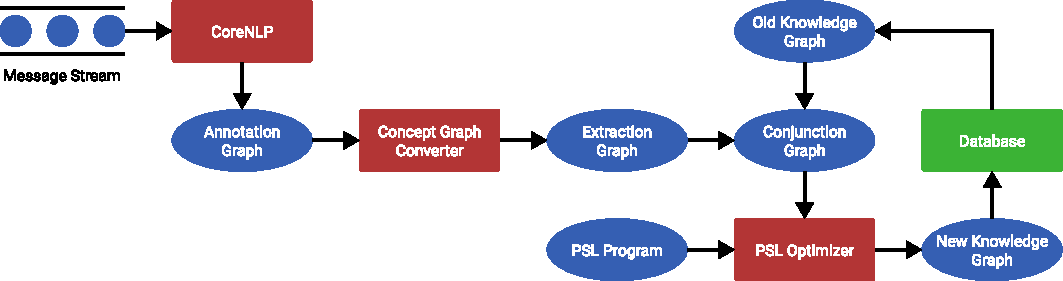
\includegraphics[width=\textwidth]{gfx/text2kg/architecture.pdf}
	\caption{Grobes Architekturdiagramm der Konstruktionspipeline}\label{fig:text2kg:architecture}
\end{figure}
Das im Folgenden vorgestellte Verfahren folgt einem dreistufigen Pipeline-Modell:
\begin{enumerate}
	\item Mittels CoreNLP wird eine eintreffende Textnachricht in einen Abhängigkeitsgraphen transformiert.
	\item Der resultierende Abhängigkeitsgraph wird in einen sog.\ Extraktionsgraphen umgewandelt.
		Hierbei handelt es sich um einen Konzeptgraphen, der den Inhalt der Nachricht formal repräsentiert.
	\item Der Extraktionsgraph wird mit dem bestehenden Wissensgraphen verschmolzen.
		Dies entspricht der Konjuktion der durch die beiden Graphen repräsentierten logischen Ausdrücke.
		Der resultierende Konjunktionsgraph wird als Eingabe für ein PSL-Programm verwendet, welches auf Basis des hinzugekommenen Wissens neue Beziehungen im Wissensgraphen inferiert.
\end{enumerate}
Die Beschreibung dieser Pipeline erfolgt in vier Abschnitten.
In \treft{sec:text2kg:implementation} wird kurz die technische Umsetzung erläutert.
\treft{sec:text2kg:ontology} beschreibt anschließend die Ontologie der konstruierten Wissensgraphen.
Nach diesen strukturellen Betrachtungen wird schließlich in \treft{sec:text2kg:nlp} und \treft{sec:text2kg:psl} die Transformation von Text zu Extraktionsgraph, bzw.\ von Extraktionsgraph zu Wissensgraph beschrieben.

\section{Implementation}%
\label{sec:text2kg:implementation}

Das in den folgenden Abschnitten beschriebene Verfahren wurde im Rahmen dieser Arbeit prototypisch implementiert.
Bei der Wahl der hierfür verwandten Technologien wurde darauf Wert gelegt, dass eine möglichst nahtlose Integration der Komponenten möglich ist.
Sowohl CoreNLP~\cite{CoreNLP} als auch die PSL-Referenzimplementation~\cite{PSL} sind JVM-Bibliotheken.
Diese Arbeit wurde daher ebenfalls in einer JVM-Sprache implementiert.

Hierfür wurde Clojure gewählt, ein moderner Lisp-1-Dialekt, mit einem Fokus auf funktionale Programmierung, unveränderliche Datenstrukturen und gleichzeitiger Interoperabilität mit objektorientierten Bibliotheken.
Andere JVM-Sprachen, wie z.~B. Java, Scala oder Groovy, wurden ausgeschlossen, da sie sich während des Entwicklungsprozesses als hinderlich erwiesen haben.
Der Hauptgrund hierfür ist, dass CoreNLP bei der Initialisierung diverse Modelle laden muss.
Bei Verwendung eines modernen Desktop-Rechners benötigt dies ca.~20 Sekunden, auf langsamerer Hardware teils mehrere Minuten;
diese Wartezeiten waren ein stark verlangsamender Faktor beim entwickeln.
Da Clojure ein Lisp ist, unterstützt es traditionsgemäß \textit{REPL Driven Development}.
Statt nach jeder Änderung die Anwendung neu zu starten und die Modelle erneut zu laden, kann so lediglich der geänderte Bytecode in den laufenden Prozess injiziert werden;
die geladenen Modelle bleiben dabei im Speicher und die Änderung kann ohne weitere Wartezeit getestet werden.
Durch die Wahl von Clojure konnte die Entwicklung deutlich beschleunigt werden.

\section{Wissensgraphontologie}%
\label{sec:text2kg:ontology}

Bevor Wissensgraphen konstruiert werden können, muss spezifiziert sein, wie genau diese aussehen sollen.
Um komplexe logische Beziehungen ausdrücken zu können, wird die bereits vorgestellte Konzeptgraph-Struktur verwendet.
Dabei bleibt allerdings offen, welche Prädikate vorkommen können und welche Bedeutung sie haben.
Außerdem ist unklar, wie mit Konzeptgraphen modale Aussagen ausgedrückt werden.
Damit aus einem Konzeptgraphen ein Wissensgraph wird, muss eine Ontologie gegeben sein, welche diese offenen Punkte schließt.
Im Folgenden wird beschrieben, wie genau die in dieser Arbeit verwendete Ontologie aufgebaut ist.

\subsection{Verwendete Prädikate}%
\label{sec:text2kg:ontology:pred}

Im ersten Schritt wird geklärt, welche Prädikate in den in dieser Arbeit konstruierten Wissensgraphen vorkommen können.
Es ist nicht sinnvoll beliebige Prädikate zuzulassen, da für eine effiziente maschinelle Weiterverarbeitung der Wissensgraphen, eine Semantik für alle vorkommenden Prädikate definiert sein muss.
Für die Wissensgraphen in dieser Arbeit wird daher eine Menge von fünf Prädikaten verwendet.

\paragraph{Syntax}
Bevor diese Prädikate näher erläutert werden, wird allerdings die Konzeptgraphsyntax leicht modifiziert.
Da alle verwendeten Prädikate entweder unär oder binär sein werden, kann eine kompaktere Notation benutzt werden:
\begin{align*}
	\vcenter{\hbox{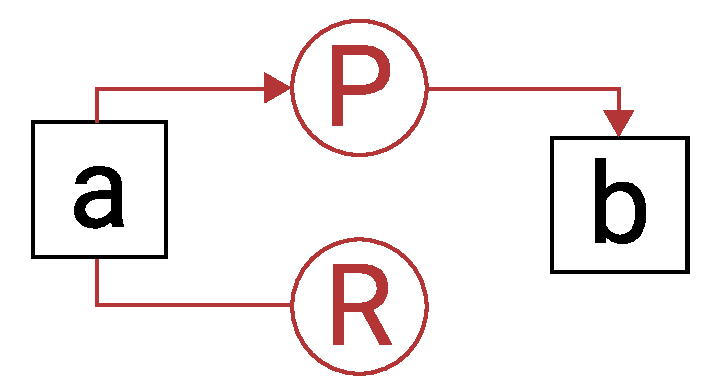
\includegraphics[scale=0.23]{gfx/text2kg/relationNodeAlternativeSyntax1.pdf}}}
	\Leftrightarrow
	\vcenter{\hbox{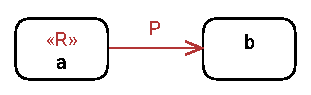
\includegraphics[scale=0.8]{gfx/text2kg/relationNodeAlternativeSyntax2.pdf}}}
\end{align*}
Relationsknoten werden nicht mehr dargestellt.
Bei unären Relationen werden die Relationsknotenbezeichner stattdessen mit in die Konzeptknoten geschrieben.
Binäre Relationen werden durch eine bezeichnete Kante zwischen dem ersten und zweiten Argument repräsentiert.

\paragraph{Wissensmodell}
Um eine semantisch konsistente Menge von Wissensgraph-Prädikaten zu definieren, ist es sinnvoll zuvor ein Modell zu definieren, welches den abstrakten Begriff des \textit{Konzeptes} formalisiert.
Konzepte sind das zentrale Syntaxelement in Konzeptgraphen;
ähnlich wie Variablen in der Prädikatenlogik, haben sie jedoch keine inhärente Bedeutung.

Im Folgenden wird ein Konzept $x$ durch eine Eigenschaftsmenge $prop(x) = \{ p_1, \dots, p_n \}$ spezifiziert.
Prädikate die für $x$ gelten bzw.\ nicht gelten, beschreiben Eigenschaften von $prop(x)$.
Es ist unrealistisch $prop(x)$ mittels Prädikaten vollständig zu definieren, da dies gleichbedeutend mit einer exakten formalen Beschreibung jedes beliebigen Konzeptes $x$ wäre.
Das Ziel ist daher stattdessen, die Eigenschaftsmengen von Konzepten in Relation zueinander zu beschreiben.
Der Wissensgraph ist also ein Formalismus zur Beschreibung von Eigenschaften der Eigenschaftsmengen von Konzepten.

\paragraph{Prädikate}
Abhängig davon, welche Eigenschaften erfasst werden sollen, können die zu verwendenden Prädikate stark variieren.
Die für diese Arbeit verwendete Prädikatsmenge hat nicht das Ziel der Vollständigkeit, sondern versucht vielmehr einige wesentliche Eigenschaften natürlichsprachlicher Aussagen zu erfassen.
Gemäß dieser Prämisse wurden fünf Wissensgraph-Prädikate definiert.
\begin{enumerate}
	\item \textbf{$label \subseteq \text{concept} \times \text{string}$:}
		Das $label$-Prädikat wird benutzt, um den Bezeichner eines Konzeptes zu repräsentieren.
		Jedes Konzept hat höchstens einen Bezeichner.
		Da Konzepte aus natürlichsprachlichen Texten extrahiert werden, kann i.~d.~R. allen Konzepten ein solcher Bezeichner zugeordnet werden.
		In der bisher verwendeten Konzeptgraphsyntax lassen sich derartige Konstanten allerdings nicht ausdrücken.
		Die Syntax wird daher erneut leicht modifiziert.
		Das $label$ eines Konzeptes wird nun, statt des Variablenbezeichners, in den zugehörigen Konzeptknoten geschrieben.
		\begin{align*}
			\vcenter{\hbox{
\includegraphics[scale=0.6]{gfx/text2kg/label.pdf}}}
			\Leftrightarrow
			\exists x: {\color{rot}label(x, \text{``book''})}
		\end{align*}
	\item \textbf{$inst \subseteq \text{concept}^2$:}
		Die $inst$-Beziehung zwischen Konzepten entspricht grob der \textit{IS-A}-Beziehung semantischer Netze.
		Das Vorhandensein von $inst(x, y)$ impliziert, dass $prop(x) \subseteq prop(y)$ gilt;
		$inst$ ist also reflexiv und transitiv.
		\begin{align*}
			\textit{``the good book''}
			\Rightarrow
			\vcenter{\hbox{
\includegraphics[scale=0.6]{gfx/text2kg/inst.pdf}}}
		\end{align*}
	\item \textbf{$relation \subseteq \text{concept}$:}
		Da die Prädikatsmenge eingeschränkt ist, können keine eigenen Prädikate für Worte eingeführt werden, die Konzepte in Relation zueinander setzen (z.~B. \textit{X likes Y}).
		Stattdessen werden sog.\ Relationskonzepte verwendet, d.~h.\ Konzepte, die andere Konzepte zueinander in Beziehung setzen.
		Relationskonzepte $r$ werden durch das unäre Prädikat $relation(r) \Leftrightarrow `relation \in prop(r)$ gekennzeichnet.
		Um die durch $r$ zueinander in Beziehung gesetzten Konzepte zu beschreiben werden die Prädikate $agent$ und $patient$ verwendet.
	\item \textbf{$agent \subseteq \text{concept}^2$:}
		Das $agent$-Prädikat zwischen einem Konzept $x$ und dem sog.\ Agens $y$ wird benutzt, um eine kausale Abhängigkeit des $x$ von $y$ zu beschreiben.
		$agent(x, y) \Leftrightarrow (`cause, y) \in prop(x)$ sagt also aus, dass $x$ aufgrund von $y$ existiert.
	\item \textbf{$patient \subseteq \text{concept}^2$:}
		Der Patiens $y$ eines Konzeptes $x$ ist ein Konzept, dessen Eigenschaften durch $x$ verändert werden.
		Es wird dabei davon ausgegangen, dass $x$ eine Eigenschaft $p_x \in prop(x)$ hat, die beschreibt, wie $x$ andere Konzepte verändert.
		$patient(x, y)$ impliziert, dass $prop(y)$ die durch $p_x$ geforderten Eigenschaften hat.
		$p_x$ lässt sich für natürlichsprachliche Konzepte offensichtlich nicht sinnvoll formal definieren.
		Dies ist allerdings auch nicht notwendig, wenn $p_x$ als von außen gegebenes Domänenwissen betrachtet wird, welches erst bei der Interpretation der Daten eingebracht wird.
\end{enumerate}
Diese Kombination von Prädikaten hat sich als hinreichend mächtig erwiesen, um eine Vielzahl natürlichsprachlicher Aussagen abzubilden.
\begin{align*}
	\textit{``I saw you yesterday.''}
	\Rightarrow
	\vcenter{\hbox{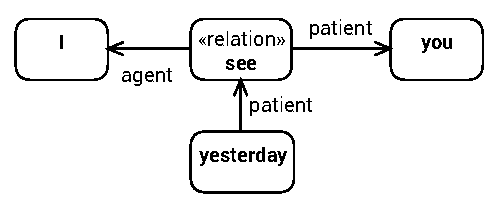
\includegraphics[scale=0.6]{gfx/text2kg/relAgPat.pdf}}}
\end{align*}

\subsection{Modale Kontexte}%
\label{sec:text2kg:ontology:modal}

Nachdem nun die verwendeten Prädikate beschrieben wurden, wird im zweiten Schritt geklärt, wie Wissensgraphen Modalität repräsentieren.
Beispiele für modale Aussagen sind:
\begin{center}
	\textit{``I {\color{blau}think} that {\color{rot}the book is good}.''}\\
	\textit{``{\color{rot}I} {\color{blau}don't want} to {\color{rot}see you}.''}
\end{center}
Die beiden Teilaussagen \textit{\color{rot}``the book is good''} und \textit{\color{rot}``I see you''} sind offensichtlich nicht unbedingt wahr, sondern beschreiben Möglichkeiten, die in Abhängigkeit von \textit{\color{blau}think} bzw.\ \textit{\color{blau}don't want} wahr oder falsch werden könnten.
Ob die Aussagen wahr werden, hängt davon ab, inwiefern das Denken oder Wollen einer Person mit der Realität --- auch aktuale Welt genannt --- übereinstimmt.
Dies ist je nach Person stark verschieden; manche tendieren dazu die allgemein als wahr akzeptierten Aussagen zu denken bzw.\ entsprechend ihrer Wünsche zu handeln, andere nicht.

Um derartige Möglichkeiten und Notwendigkeiten direkt zu repräsentieren, reichen die vorgestellten Konzeptgraphen mit Negationskontexten nicht aus.
Sowa hat dieses Problem ebenfalls erkannt und daher weitere Kontexttypen eingeführt.
Die Beschreibung dieser zusätzlichen Kontexttypen ist allerdings oftmals zu unpräzise für eine eindeutige Übersetzung in die Prädikatenlogik.
Aufbauend auf Sowas Ideen wird in dieser Arbeit daher eine Variante modaler Kontexte eingeführt, die die Übersetzbarkeit in die Prädikatenlogik erster Ordnung bewahrt.
Da die zuvor vorgestellten Konzeptgraphen bereits vollständig und korrekt sind, handelt es sich bei diesen modalen Kontexten also lediglich um eine Kurzschreibweise.

Insgesamt gibt es durch die Erweiterung um modale Kontexe nun folgende vier Kontexttypen:
\begin{multicols}{2}
	\flushleft\begin{enumerate}
		\item Positiver Aktualkontext
		\item Negativer Aktualkontext
		\item Positiver Möglichkeitskontext
		\item Negativer Möglichkeitskontext
	\end{enumerate}
\end{multicols}
Die modale Notwendigkeit hat keine eigenen Kontexttypen erhalten, um konsistent zur Quantisierung in Konzeptgraphen zu bleiben.
So, wie der Allquantor in Konzeptgraphen durch Negation der negierten existenzquantisierten Aussage ausgedrückt wird, wird die Notwendigkeit durch Negation der negativen Möglichkeit ausgedrückt.

Da es nun vier Kontexttypen gibt, muss die Konzeptgraphsyntax leicht angepasst werden, um zwischen den verschiedenen Typen differenzieren zu können:
\begin{figure}[h]
	\centering
	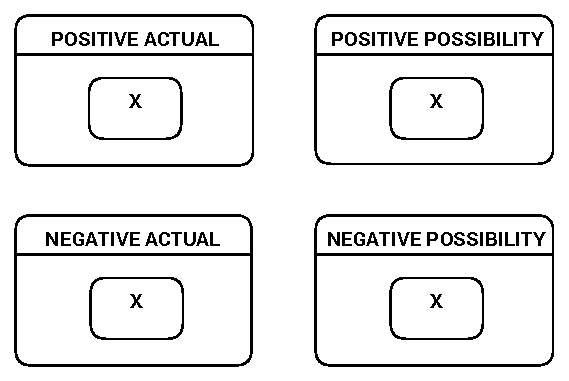
\includegraphics[scale=0.6]{gfx/text2kg/contextTypes.pdf}
	\caption{Konzeptgraphsyntax für modale Kontexte}\label{fig:text2kg:contextTypes}
\end{figure}

\paragraph{Positiver Aktualkontext}
Dieser Kontexttyp hat keinen Einfluss auf die Bedeutung der enthaltenen Knoten.
Er entspricht in etwa der Klammerung in der Prädikatenlogik.
Das \textit{Sheet of Assertion}~$\top$ ist ein solcher Kontext, abgesehen davon tauchen positive Aktualkontexte allerdings nicht auf;
sie werden hier lediglich der Vollständigkeit halber erwähnt.
\begin{align}
	\vcenter{\hbox{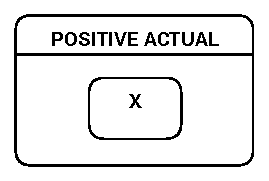
\includegraphics[scale=0.6]{gfx/text2kg/positiveActual.pdf}}}
	\Leftrightarrow
	\vcenter{\hbox{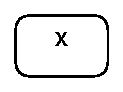
\includegraphics[scale=0.6]{gfx/text2kg/x.pdf}}}
	\Leftrightarrow
	\exists x: label(x, \text{``X''})
\end{align}

\paragraph{Negativer Aktualkontext}
Entspricht dem bisherigen Negationskontext.
\begin{align}
	\vcenter{\hbox{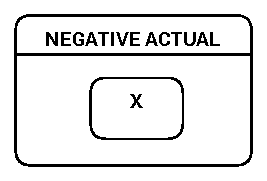
\includegraphics[scale=0.6]{gfx/text2kg/negativeActual.pdf}}}
	\Leftrightarrow
	\lnot \exists x: label(x, \text{``X''})
\end{align}

\paragraph{Positiver Möglichkeitskontext}
Dieser Kontexttyp bildet die modale Möglichkeit ab.
Um die Mächtigkeit der Prädikatenlogik beizubehalten, wird hierfür keine fundamental neue Struktur eingeführt.
Es wird stattdessen die Tatsache ausgenutzt, dass sich die modalen Operatoren gemäß der Mögliche-Welten-Interpretation analog zu den prädikatenlogischen Quantoren verhalten.
\begin{align*}
	{\color{rot}\square} P(x)\ &\Leftrightarrow \lnot {\color{blau}\lozenge} \lnot P(x) \\
	{\color{rot}\forall} w: world(w) \rightarrow P_w(x)\ &\Leftrightarrow \lnot {\color{blau}\exists} w: world(w) \land \lnot P_w(x) \numberthis
\end{align*}
Die Aussage \textit{``$P(x)$ gilt notwendigerweise''}, wird also als \textit{``Es gibt keine Welt $w$ in der $P_w(x)$ nicht gilt''} aufgefasst.
Statt von Welten, wird in modalen Konzeptgraphen allerdings von Kontexten gesprochen.
\begin{align*}
	\vcenter{\hbox{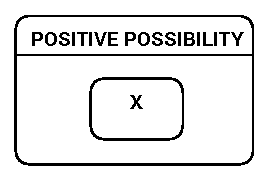
\includegraphics[scale=0.6]{gfx/text2kg/positivePossib.pdf}}}
	&\Leftrightarrow
	\vcenter{\hbox{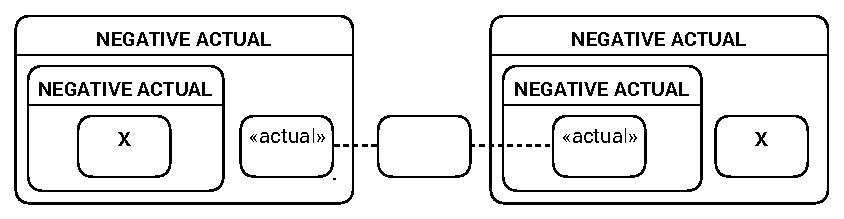
\includegraphics[scale=0.6]{gfx/text2kg/possibExpansion.pdf}}} \numberthis \\
	&\Leftrightarrow
	\exists c: context(c) \land (actual(c) \leftrightarrow \exists x: label(x, \text{``X''}))
\end{align*}
Anders als Aktualkontexte, tauchen Möglichkeitskontexte explizit in der prädikatenlogischen Repräsentation auf, sie lassen sich also nicht nur als Kontext sondern zugleich auch als Konzept auffassen.
Der in einem Möglichkeitskontext $c$ enthaltene Teilgraph $G$ ist dabei genau dann wahr, wenn der Kontext die aktuale Welt beschreibt~($\Leftrightarrow actual(c)$).
Solange $actual(c)$ unbekannt ist, kann also keine Aussage über die Wahrheit von $G$ gemacht werden.
Wenn $actual(c)$ jedoch wahr bzw.\ falsch ist, ist $c$ äquivalent zu einem positiven bzw.\ negativen Aktualkontext.

Zur Bestimmung von des Wahrheitswertes von $actual(c)$ ist i.~d.~R. domänenspezifisches Wissen notwendig.
Dieses domänenspezifische Wissen, kann durch sog.\ Kontextrelationen eingebracht werden.
Da Möglichkeitskontexte zugleich Konzepte sind, lassen sie sich zu anderen Konzepten in Relation setzen.
Dies ist z.~B. dann nützlich, wenn man die Aussage \textit{``I {\color{blau}think} that {\color{rot}the book is good}.''} repräsentieren möchte.
\begin{align*}
	&\vcenter{\hbox{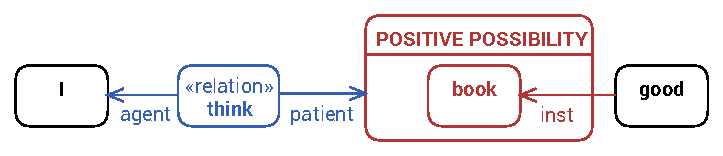
\includegraphics[scale=0.6]{gfx/text2kg/possibCtxRelationExample.pdf}}} \numberthis \\
	\Leftrightarrow
	\exists i, g, t, c:&\ label(i, \text{``I''}) \land label(g, \text{``good''}) \\
	\land&\ {\color{blau}label(t, \text{``think''}) \land relation(t) \land agent(t, i) \land patient(t, c)} \\
	\land&\ {\color{rot}context(c) \land (actual(c) \leftrightarrow \exists b: label(b, \text{``book''}) \land inst(g, b))}
\end{align*}
Durch die Verknüpfung $patient(t, c)$ eines Konzeptes mit einem Kontext, kann Wissen über das Konzept benutzt werden, um Schlüsse über die Aktualität des Kontextes zu ziehen.
Wie genau dies ablaufen kann, ist bislang allerdings noch unklar.
In~\treft{sec:text2kg:psl} wird die $actual$-Inferenz näher untersucht.

\paragraph{Negativer Möglichkeitskontext}
Lediglich eine Kurzschreibweise für einen positiven Möglichkeitskontext der einen negativen Aktualkontext umgibt.
\begin{align}
	\vcenter{\hbox{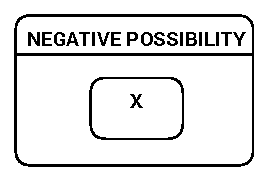
\includegraphics[scale=0.6]{gfx/text2kg/negativePossib.pdf}}}
	\Leftrightarrow
	\vcenter{\hbox{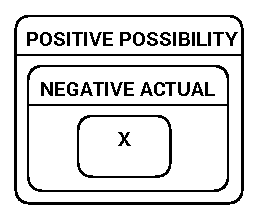
\includegraphics[scale=0.6]{gfx/text2kg/negativePossibExpansion.pdf}}}
\end{align}

\section{NLP-Phase}%
\label{sec:text2kg:nlp}

\section{Graphkonstruktionsphase}%
\label{sec:text2kg:psl}

% !TEX root = ../main.tex
% chktex-file 46
\chapter{Bewertung}%
\label{sec:evaluation}

Die Bewertung des im vorigen Kapitel vorgestellten Verfahrens erfolgt in zwei Schritten.
In~\ref{sec:evaluation:quality} wird im ersten Schritt die Qualität der konstruierten Wissensgraphen untersucht.
Anschließend wird in~\ref{sec:evaluation:time} die Tauglichkeit des Verfahrens im Kontext von Nachrichtenstreams betrachtet.

\section{Qualitative Bewertung}%
\label{sec:evaluation:quality}

Das vorgestellte Verfahren macht zahlreiche Annahmen über die Struktur und Komplexität der Eingabedaten, zudem wird lediglich ein kleiner Teil aller potentiell in Annotationsgraphen enthaltenen Informationen genutzt.
In diesem Kapitel wird betrachtet, wie sich diese Einschränkungen auf die Qualität der resultierenden Wissensgraphen auswirken.
Ziel ist dabei nicht eine umfassende empirische Auswertung durchzuführen, sondern stattdessen die Stärken und Schwächen des Verfahrens anhand von stichprobenartig ausgewählten, realen Beispieldaten aufzuzeigen.
Es gibt im Wesentlichen drei Gründe für diese Entscheidung:
\begin{enumerate}
	\item Das entwickelte Verfahren ist primär prototypisch zu verstehen.
		Das Ziel war nicht ein bestimmtes Maß an Qualität zu erreichen, sondern vielmehr die Praktikabilität des Ansatzes zu demonstrieren.
	\item Es gibt keine alternativen Ansätze mit dem das entwickelte Verfahren verglichen werden kann.
		Eine automatisierte Konzeptgraph-basierte Wissensgraph-Konstruktion aus natürlichsprachlichen Nachrichten wurde bislang in keiner anderen Arbeit untersucht.
	\item Es existieren zudem keine Testdatensets, die für eine empirische Analyse des entwickelten Verfahrens geeignet sind.
		Es existieren zwar Testdaten für die verwendeten NLP-Tasks (NER, POS-Tagging, Coreference Resolution etc.), da die Ergebnisse hierfür allerdings direkt aus CoreNLP stammen, würde mit den verfügbaren Testdaten lediglich die Performance von CoreNLP gemessen.
		Benötigt wären Testdaten, die das Evaluieren der Konzept\-graph\-struktur erlauben, d.~h.\ solche, die Informationen über die semantischen Abhängigkeiten und Negation von Konzepten enthalten.
\end{enumerate}

\subsection{Bewertungsansatz}%
\label{sec:evaluation:quality:method}

Da für die Bewertung nicht auf Referenzergebnisse zurückgegriffen werden kann, müssen die Ergebnisse manuell ausgewertet werden.
Das manuelle Auswerten einer repräsentativen Stichprobe von Testnachrichten hätte den zeitlichen Rahmen dieser Arbeit gesprengt.
Daher wird stattdessen mit einer kleinen Menge von Testnachrichten gearbeitet.
Um das Ergebnis dieser Nachrichten zu bewerten, wird der aus ihnen konstruierte Wissensgraph im ersten Schritt in eine Neo4j-Graphdatenbank~\cite{Neo4j} eingefügt.
Anschließend wird daran eine Menge von Testanfragen~\tref{sec:appendix:queries} gestellt und die Ergebnisse manuell mit den in den Nachrichtentexten enthaltenen Informationen abgeglichen.
Auf diesem Wege kann zwar die Wissensgraphqualität nicht akkurat beurteilt werden, es ist allerdings möglich tendenzielle Stärken und Schwächen des Verfahrens zu erkennen.

\subsection{Testdaten}%
\label{sec:evaluation:quality:data}

Die verwendeten Textnachrichten stammen aus dem Enron E-Mail Datenset~\cite{Cohen2015}.
Da das zufällige Auswählen von E-Mails aus diesem Datenset i.~d.~R. in unzusammenhängenden Nachrichtensets resultiert, wurden die Enron Daten nicht direkt benutzt, sondern stattdessen der Enron Threads Corpus~\cite{Jamison2013}\cite{EnronThreads}.
Hierbei handelt es sich um ein Datenset, welches die E-Mail-Rohdaten in zusammengehörige Kommunikationsthreads gruppiert.
Die Nachrichten innerhalb eines Threads sind gut als Testdaten geeignet, da darin oftmals dieselben Personen und Themen auftauchen und somit die Möglichkeit besteht, Beziehungen zwischen diesen zu finden.

Für die Testnachrichten wurde zufällig ein Testthread aus der Menge aller Threads ausgewählt, der die Schlüsselwörter \textit{``yesterday''} oder \textit{``tomorrow''} enthält.
Ziel dabei war es, Nachrichten, in denen es um Termine oder Ereignisse geht, zu erhalten, da diese Nachrichten häufig auch ohne umfangreiches domänenspezifisches Wissen verstanden werden können.
Die Wahl eines beliebigen Threads resultierte meist in Nachrichten, die nur mit domänenspezifischem Wissen aus der Energie-Branche verständlich sind.
Die konkret verwendeten Testnachrichten sind in~\ref{sec:appendix:msgs} zu finden.

\subsection{Ergebnisse}%
\label{sec:evaluation:quality:results}

In diesem Abschnitt wird der aus den Testdaten konstruierte Wissensgraph\footnote{Es befindet sich ein Neo4j-Datenbank-Export des Wissensgraphen unter \url{https://github.com/Cortys/bachelor-thesis/blob/master/thesis/data/evaluation/testKG.cql}, mit diesem können die Ergebnisse nachvollzogen werden.} untersucht.
Hierfür werden vier Testanfragen benutzt.
Die Ergebnisse dieser Anfragen werden auf Korrektheit geprüft und benutzt, um Verbesserungspotential des Verfahrens aufzuzeigen.
Dabei wird zwischen zwei Arten von Fehlern unterschieden:
\newcommand{\errorA}{{\color{rot} (A)}}
\newcommand{\errorB}{{\color{blau} (B)}}
\begin{tasks}[label-offset=1em](2) % chktex 36
	\task[\errorA] \color{rot}Fehlerhafte Informationen
	\task[\errorB] \color{blau}Fehlende Informationen
\end{tasks}

\paragraph{Personen}
Die erste Anfrage~\tref{sec:appendix:queries:people} testet, welche Personen in den Nachrichten erkannt wurden.
Da dieselbe Person in verschiedenen Kontexten verschiedene Namen haben kann, ist die Ausgabe der Anfrage eine Liste von Personen, die jeweils durch eine Liste von Namen beschrieben werden.
\csvautobooklongtable[separator=semicolon]{data/evaluation/people.csv}
In den Testnachrichten werden fünf Personen erkannt.
Dabei lassen sich zwei Fehler beobachten:
\begin{enumerate}
	\item Es kommen nur vier Personen in den Nachrichten vor.
		Der Bezeichner \textit{Dr. Lu} von Person~5 wurde nicht als koreferent zu den Bezeichnern von Person~1 erkannt. % chktex 12
		Dies liegt daran, dass für die Erkennung von koreferenten Namen lediglich die CoreNLP Koreferenzinformationen und die Jaro-Distanzen von $named$-Konzepten berücksichtigt werden.
		Das Ergebnis ließe sich verbessern, indem weitere Informationen, wie z.~B. der Kontext, in dem ein Bezeichner auftaucht berücksichtigt werden. \errorB\
	\item Person~1 hat die drei fehlerhaften Bezeichner \textit{TX Zimin}, \textit{address} und \textit{Zimin Lu Enron Corp} erhalten.
		Diese Fehler stammen aus dem Dependency Parser von CoreNLP, sie lassen sich mit der aktuellen Architektur, in der alle Informationen über den Eingabetext aus den CoreNLP-Annotatoren stammen, also nicht vermeiden.
		Die Ursache des Fehlers ist die Testnachricht~6~\tref{sec:appendix:msgs}, in der eine Postanschrift vorkommt;
		damit kann CoreNLP in der verwendeten Version~3.8.0 noch nicht umgehen. \errorA\
\end{enumerate}

\paragraph{Ereignisse und Termine}
Die zweite Anfrage~\tref{sec:appendix:queries:events} testet, wie gut $relation$-Konzepte erkannt werden.
Hierfür wird aufgelistet, was \textit{Duane Seppi} wann getan hat.
\csvautobooklongtable{data/evaluation/personTimeAction.csv}
Wie zu erwarten, finden sich im Ergebnis für alle gesendeten und empfangenen Nachrichten entsprechende \textit{send}- bzw. \textit{receive}-Einträge.
Unter den übrigen Einträgen, wurden den ersten beiden Einträgen Zeitpunkte zugeordnet.
Beide stammen aus der ersten Testnachricht und sind im Wesentlichen korrekt, die relativen Zeitangaben \textit{yesterday} und \textit{today} wurden von SUTime korrekt aufgelöst und die PSL-Regel \ruleref{rule:text2kg:i} hat die Pronomina, die Agens der $relation$-Konzepte sind, korrekt der Person \textit{Duane Seppi} zugeordnet.
Es wurden allerdings auch verschiedene Fehler gemacht:
\begin{enumerate}
	\item In den Einträgen 8 und 9 haben Fehler im Abhängigkeitsgraphen eine semantisch inkorrekte Repräsentation des ersten Satzes von Nachricht~3 verursacht:
	 	\textit{``I would be grateful if I could talk with you some time about the typical terms one sees in Swing, take or pay, virtual storage, etc.\ options.''} \errorA\
	\item Die Einträge 15 und 16 sind fehlerhaft, da bei der CoreNLP Coreference Resolution das Pronomen \textit{I} des zweiten Satzes von Nachricht~6 fälschlicherweise mit \textit{Duane Seppi} verknüpft wurde. \errorA\
	\item Die Aussage von Satz~2 aus Nachricht~3 wird nicht im Wissensgraphen repräsentiert:
		\textit{``This is related to some research some colleagues and I are doing applying recent innovations in Monte Carlo valuation of options with early exercise.''} \errorB\

		Der Grund hierfür ist, dass nicht alle Universal Dependencies Abhängigkeitstypen auf ihre semantische Entsprechung in der Wissensgraphontologie abgebildet werden.
		Der obige Satz wird z.~B. deshalb nicht korrekt im Graphen repräsentiert, da die Abhängigkeitstypen \texttt{advcl} und \texttt{acl} bislang nicht berücksichtigt werden.
\end{enumerate}

\paragraph{Personenbezogene Daten}
Die dritte Anfrage~\tref{sec:appendix:queries:numbers} testet, wie gut Faktenwissen, welches in der Eingabe vorhanden ist, erkannt und aus dem Wissensgraphen ausgelesen werden kann.
In den verwendeten Testnachrichten teilen sich zwei Personen ihre Telefonnummern mit.
Die Anfrage nach allen Nummern und zugehörigen Nummertypen (Telefon-, Fax-, Hausnummer etc.) aller Personen, liefert folgendes Ergebnis:
\csvautobooklongtable[separator=semicolon]{data/evaluation/numbers.csv}
Die Telefonnummern wurden korrekt erkannt.
Bei der ersten Nummer fehlt jedoch die Information, dass es sich um eine Telefonnummer handelt \errorB;\@
dies liegt daran, dass in der Nachricht, in der sie vorkommt nicht explizit erwähnt wird, um was für eine Art Nummer es sich handelt.
Um dies zu erkennen, müssten Kommunikationsverläufe berücksichtigt werden, statt Nachrichten weitestgehend isoliert zu betrachten.

\paragraph{Positive und negative Aussagen}
In den vorigen Anfragen wurden Kontexte nicht berücksichtigt, da die Testnachrichten größtenteils Tatsachen beschreiben.
Die vierte Anfrage~\tref{sec:appendix:queries:neg} wird daher benutzt, um die Erkennung von Negationskontexten zu testen.
Konkret werden hierfür alle Relationen abgefragt, die in von \textit{John Doe} geschriebenen Nachrichten erwähnt werden und für die etwas über deren Wahrheit oder Unwahrheit bekannt ist.
\csvautobooklongtable[separator=semicolon]{data/evaluation/personNegationAction.csv}
Relation~2 wurde dabei semantisch inkorrekt abgebildet \errorA.
Die Negation von \textit{``I have something''} im Satz \textit{``I'm not writing this message because I have something to say''} wurde nicht erkannt.
Grund hierfür ist zum einen, dass der Abhängigkeitstyp \texttt{advcl} in der NLP-Phase nicht berücksichtigt wird.
Außerdem fehlt das Hintergrundwissen über die Bedeutung des Wortes \textit{because}.
Um den Satz korrekt zu verstehen, wäre es notwendig die Implikation $\textit{I have something} \rightarrow \lnot(\textit{I write message})$ zu erkennen, mit dem Wissen, dass \textit{I write message} wahr ist, zu verknüpfen und schließlich $\lnot(\textit{I have something})$ zu folgern.
Zu derartige Schlussfolgerungen ist das vorgestellte Verfahren bislang nicht in der Lage.

\section{Laufzeituntersuchung}%
\label{sec:evaluation:time}

In diesem Abschnitt wird untersucht, inwiefern sich das beschriebene Verfahren im Kontext von Nachrichtenstreams eignet.
Da in der PSL-Phase für jede eingefügte Nachricht momentan eine vollständige ADMM-basierte Inferenz durchgeführt wird, ist zu erwarten, dass mit jeder eingefügten Nachricht die Inferenzdauer steigt.

% !TEX root = ../main.tex
% chktex-file 46
\chapter{Zusammenfassung}%
\label{sec:conclusion}

Abschließend wird nun zusammengefasst, inwiefern das in~\ref{sec:intro:goals} beschriebene Ziel einer erweiterbaren, parallelisierbaren Wissensgraph-Konstruktion aus Kommunikationsdaten erreicht wurde.
Hierfür werden in~\ref{sec:conclusion:review} die erreichten Teilziele betrachtet.
Anschließend wird in~\ref{sec:conclusion:todo} ein Ausblick auf Möglichkeiten der Weiterentwicklung des Systems gegeben.

\section{Rückblick}%
\label{sec:conclusion:review}

\begin{figure}[h]
	\centering
	
\includegraphics[width=0.65\textwidth]{gfx/conclusion/overview.pdf}
	\caption{Grober Aufbau des Konstruktionsverfahrens}\label{fig:conclusion:overview}
\end{figure}
In Kapitel~\ref{sec:text2kg} wurden Lösungen für die drei wesentlichen Teilprobleme Ontologie, Sprachverarbeitung und Grapherweiterung beschrieben.
Die drei Teillösungen bilden zusammen ein Konstruktionsverfahren, welches dem zu Anfang beschriebenen Aufbau entspricht.

\paragraph{Ontologie}
Die Wissensgraphontologie basiert auf Konzeptgraphen.
Im Gegensatz zu den Fakten-Tripel basierten semantischen Netzen, die lediglich beschreiben, welche Beziehungen zwischen Konzepten existieren, kann mittels Konzeptgraphen auch beschrieben werden, welche Beziehungen nicht, oder nur möglicherweise existieren.
Die konstruierten Wissensgraphen haben also eine deutlich höhere Ausdrucksstärke, als z.~B. NELL oder der Google~Knowledge~Graph.
Diese Ausdrucksstärke ist wichtig, um die Komplexität natürlichsprachlicher Aussagen abbilden zu können.

Damit den konstruierten Konzeptgraphen eine Semantik zugeordnet werden, muss die Semantik der verwendeten Relationen beschrieben werden.
Es wurde daher ein möglichst minimales Set von Relationen definiert~\tref{sec:text2kg:ontology:pred}, welches zur Beschreibung einer Vielzahl natürlichsprachlicher Aussagen geeignet ist.

Eine der in~\ref{sec:intro:goals} beschriebenen Anforderungen an das Konstruktionsverfahren ist die Erweiterbarkeit, d.~h.\ die prinzipielle Möglichkeit nicht natürlichsprachliche Eingaben einzufügen.
Konkret bedeutet dies, dass z.~B. ein Bild in denselben Wissensgraph eingefügt werden kann, in den auch Textnachrichten eingefügt werden.
Da die gewählten Konzeptgraph-Relationen nicht speziell für natürliche Sprache ausgelegt sind, ist dies prinzipiell möglich;
es gibt keine Relationen, die bestimmte grammatikalische Konstrukte oder Wortarten abbilden.
Wie die Integration anderer Eingabearten im Detail aussehen könnte, war jedoch nicht Teil der Aufgabenstellung und wurde daher nicht näher untersucht.

\paragraph{Sprachverarbeitung}
Für die Transformation einer Nachricht in einen Konzeptgraphen wurde das Stanford~CoreNLP Framework mit einer Menge von Transformationsregeln~\tref{sec:text2kg:nlp:transform} kombiniert, welche die von CoreNLP gefundenen Strukturen auf äquivalente Konzeptgraph-Strukturen abbilden.

\paragraph{Grapherweiterung}
Das Einfügen des aus einer Nachricht extrahierten Konzeptgraphen in einen bestehenden Wissensgraphen erfolgt mittels PSL.\@
Im Rahmen dieser Arbeit wurde PSL erstmals im Kontext einer Konzeptgraph-basierten Wissensgraph-Konstruktion eingesetzt.
Es wurde ein Set von PSL-Regeln~\tref{sec:text2kg:psl:inference} vorgestellt, welches den Einsatz in diesem Kontext exemplarisch aufzeigt.

Neben der Erweiterbarkeit war auch die Parallelisierbarkeit eines der in~\ref{sec:intro:goals} beschriebenen Ziele.
Durch die Wahl von PSL für die Grapherweiterung wurde diese Anforderung prinzipiell erfüllt.
Das für die Inferenz verwendete ADMM-Verfahren lässt sich gut verteilt implementieren.
In~\cite[Kapitel 10]{Boyd2011} wird beschrieben, wie sich ADMM mit verteilten Programmiermodellen, wie z.~B. MapReduce oder Pregel, implementieren lässt.
Aufbauend darauf, wird in~\cite{Lubell-Doughtie2013} eine Hadoop MapReduce-basierte Implementation vorgestellt.
PSL ist prinzipiell also für den Einsatz in Cluster-Umgebungen geeignet.
Die exemplarische verteilte PSL-Implementation \textit{foxPSL}~\cite{Magliacane2015} demonstriert dies.
In der im Rahmen dieser Arbeit erstellten Implementation wurde die PSL-Referenzimplementation verwendet, da diese am besten dokumentiert ist und die Geschwindigkeit für die verwendeten kleinen Datensets ausreichend ist.

Das Ziel ein erweiterbares, parallelisierbares Wissensgraph-Konstruktionsverfahren für Kommunikationsdaten zu konzipieren wurde somit prinzipiell erreicht.
Nichts desto trotz gibt es noch zahlreiche Möglichkeiten das vorgestellte Verfahren weiterzuentwickeln.

\section{Ausblick}%
\label{sec:conclusion:todo}

Im Folgenden wird ein Überblick über Möglichkeiten der Weiterentwickung und offen gebliebene Fragestellungen gegeben.

\paragraph{Verbessern der Testmethode}
Ein Problem bei der Konzeption des Verfahrens war der Umstand, dass es keine Kommunikationsdaten mit Referenzergebnissen gibt, anhand derer Änderungen am Verfahren bewertet werden können.
Die Qualität vieler Entscheidungen, wie z.~B. der Wahl der Regelgewichte, konnte daher nur auf Basis manuell durchgeführter, stichprobenartiger Tests bewertet werden.

Um dieses Problem zu lösen, könnte ein Kommunikationsdaten-Testset entwickelt werden, mit dem sich die Performance eines Wissensgraph-Konstruktionsverfahrens repräsentativ empirisch messen lässt.
Ein solches Datenset ist wichtig, um ein systematisches Weiterentwickeln des Verfahrens zu ermöglichen.
Das in dieser Arbeit verwendete Enron E-Mail Datenset ist potentiell ein guter Ausgangspunkt hierfür.
Zu klären ist, welche Art von Informationen die Referenzergebnisse enthalten und wie eine umfangreiche Menge solcher Referenzergebnisse konstruiert werden kann.

\paragraph{NLP-Phase}
Im vorgestellten Verfahren wird lediglich ein Teil der von CoreNLP extrahierten Informationen in Konzeptgraph-Strukturen übersetzt.
Durch die Integration bislang ungenutzter Abhängigkeitstypen ließe sich die Qualität der Ergebnisse, wie in~\ref{sec:evaluation:quality:results}~Anfrage~2 gezeigt, deutlich verbessern.

Außerdem sollte die verwendete Heuristik zur Übersetzung von natürlichsprachlicher Negation in negative Kontexte verbessert werden.
In~\ref{sec:evaluation:quality:results}~Anfrage~4 wird dies deutlich.
Ein Ansatz hierfür ist z.~B. das Nutzen des CoreNLP Natural Logic Annotators~\cite{MacCartney2007}, welcher u.~a.\ Quantoren, Negationen und die zugehörigen Scopes, d.~h.\ die modifizierten Token, erkennt.

\paragraph{PSL-Phase}
Die verwendeten domänenspezifischen Regeln und das domänenspezifische Vorwissen sind bislang sehr rudimentär.
In künftigen Arbeiten könnten vorhandene Wissensbasen, wie z.~B. NELL~\cite{Carlson2010} oder YAGO~\cite{YAGO}, in die PSL-Inferenz integriert werden.

Neben der Nutzung domänenspezifischen Wissens, besteht außerdem Verbesserungspotential bei der Nutzung von Kontexten in der Inferenz.
Bislang werden Kontexte nur benutzt, um die Richtung von $inst$-Relationen zu ermitteln.
Das Inferieren des $actual$-Attributs von Möglichkeitskontexten~\tref{sec:text2kg:ontology:modal} zur Bestimmung der Glaubwürdigkeit von Aussagen wäre z.~B. eine sinnvolle Erweiterung des Verfahrens.

\paragraph{Inferenz}
Wie~\treft{sec:evaluation:time} gezeigt hat, besteht noch Verbesserungsbedarf bei der Geschwindigkeit der PSL-Inferenz, bevor das Verfahren in der Praxis einsetzbar ist.
Um dies zu erreichen, ist die Kombination verschiedener Ansätze denkbar:
\begin{enumerate}
	\item Nutzen einer Cluster-fähigen ADMM-Implementation, statt der PSL-Referenz\-implementation.
		Hierfür könnte z.~B. die zuvor erwähnte Hadoop MapReduce Implementation~\cite{Lubell-Doughtie2013} oder foxPSL~\cite{Magliacane2015} verwendet werden.
	\item Weiterentwicklung von BOCI, sodass wachsende Eingabemengen unterstützt werden.
		Bereits im ursprünglichen Paper~\cite[Abschnitt 6]{Pujara2015} wird dies als offene Fragestellung für folgende Arbeiten genannt.
		Mittels des Inferenz-Budgets könnte dann die Inferenzdauer nahezu beliebig verringert werden, sofern dafür eine entsprechende Verschlechterung der Inferenzqualität hingenommen wird.
	\item Effizienterer Umgang mit transitiven Relationen.
		Bei der Inferenz werden $inst$-Atome aufgrund der Transitivität von $inst$ instanziiert.
		Während der Inferenz sind diese Atome wichtig, sie werden momentan allerdings auch Teil des Wissensgraphen.
		Das Entfernen dieser redundanten $inst$-Atome, würde die Kantenanzahl des in~\ref{sec:evaluation:time} konstruierten Graphen um mehr als 75\% verringern.
		Während der Inferenz würden die transitiven $inst$-Relationen dann nur temporär instanziiert.
		Inwiefern durch eine derartige Erweiterung der PSL-Inferenz neben der Graph-Größe auch die Inferenzdauer verringert werden kann, ist zu untersuchen.
\end{enumerate}

Wie soeben gezeigt, gibt es viele Möglichkeiten das vorgestellten Wissensgraph-Konstruktionsverfahren weiterzuentwickeln.
Diese Arbeit ist daher primär als ein Ausgangspunkt zu verstehen, der zeigt, dass die Kombination von Konzeptgraphen, NLP und PSL prinzipiell für die automatisierte Konstruktion von Wissensgraphen geeignet ist.
Aufbauend auf dieser Grundidee könnte in künftigen Arbeiten ein in der Praxis einsetzbares Verfahren entwickelt werden.


% --------------------------
% Back matter
% --------------------------
\appendix\cleardoublepage\
% !TEX root = ../my-thesis.tex
%
\chapter{Example Appendix}
\label{sec:appendix}

\Blindtext[1][1]

\section{Appendix Section 1}
\label{sec:appendix:sec1}

\Blindtext[1][1]

\begin{table}[h]
	\begin{tabularx}{\textwidth}{X | X | X}
		%\hline
		Alpha		& Beta			& Gamma			\\ \hline
		0			& 1				& 2				\\ \hline
		3			& 4				& 5				\\ %\hline
	\end{tabularx}
	\label{tab:table1}
	\caption{This is a caption text.}
\end{table}

\section{Appendix Section 2}
\label{sec:appendix:sec2}

\Blindtext[1][1]

\begin{table}[h]
	\begin{tabularx}{\textwidth}{X | X | X}
		%\hline
		Alpha		& Beta			& Gamma			\\ \hline
		0			& 1				& 2				\\ \hline
		3			& 4				& 5				\\ %\hline
	\end{tabularx}
	\label{tab:table2}
	\caption{This is a caption text.}
\end{table}

\Blindtext[1][2]
       % INCLUDE: appendix
%
{%
\setstretch{1.1}
\renewcommand{\bibfont}{\normalfont\small}
\setlength{\biblabelsep}{0pt}
\setlength{\bibitemsep}{0.5\baselineskip plus 0.5\baselineskip}
\printbibliography[nottype=online]
\printbibliography[heading=subbibliography,title={Webseiten},type=online,prefixnumbers={@}]
}
\cleardoublepage\

\listoffigures
\cleardoublepage\

\listoftables
\cleardoublepage\

% !TEX root = ../main.tex
%
%************************************************
% Declaration
%************************************************
\pdfbookmark[0]{Declaration}{Declaration}
\chapter*{Declaration}
\label{sec:declaration}
\thispagestyle{empty}

You can put your declaration here, to declare that you have completed your work solely and only with the help of the references you mentioned.

\bigskip

\noindent\textit{\thesisUniversityCity, \thesisDate}

\smallskip

\begin{flushright}
	\begin{minipage}{5cm}
		\rule{\textwidth}{1pt}
		\centering\thesisName
	\end{minipage}
\end{flushright}

%*****************************************
%*****************************************

\clearpage
\newpage

% **************************************************
% End of Document CONTENT
% **************************************************
\end{document}
